%  compress using: gs -sDEVICE=pdfwrite -dCompatibilityLevel=1.4 -dNOPAUSE -dQUIET -dBATCH      -sOutputFile=foo-ShapingSwarmCompressed.pdf ShapingSwarmFrictionSharedInput.pdf

%\documentclass[conference]{IEEEtran}
\documentclass[letterpaper, 10 pt, conference]{ieeeconf}
\IEEEoverridecommandlockouts% This command is only needed if 
                                                          % you want to use the \thanks command
%\overrideIEEEmargins                                      % Needed to meet printer requirements.
\usepackage{times}


\makeatletter 
\let\NAT@parse\undefined
\makeatother

% numbers option provides compact numerical references in the text. 
%\usepackage[numbers]{natbib}
\usepackage{multicol}
%\usepackage[bookmarks=true]{hyperref}

\usepackage{bbm}
\usepackage{calc}
\usepackage{url}
\usepackage{transparent}
\usepackage[bookmarks=true,hidelinks]{hyperref}

\usepackage{graphicx}
\usepackage[cmex10]{amsmath}
\usepackage{bm}
\usepackage{amssymb}
\usepackage{rotating}

\usepackage{chngcntr}
\counterwithin{paragraph}{subsection} % makes paragraph depend on subsection


%\usepackage{xfrac}
\usepackage{nicefrac}
\usepackage{cite}
\usepackage[caption=false,font=footnotesize]{subfig}
\usepackage[usenames, dvipsnames]{color}
\usepackage{colortbl}
%\usepackage{caption}

%\usepackage{wrapfig}
\usepackage{overpic}
%\usepackage{subfigure}
%\usepackage{textcomp}
\graphicspath{{./pictures/pdf/},{./pictures/ps/},{./pictures/png/},{./pictures/jpg/}}
\usepackage{breqn} %for breaking equations automatically
\usepackage[ruled]{algorithm}
\usepackage{algpseudocode}
%\usepackage{algorithmic}
\usepackage{multirow}
\usepackage{todonotes}
\usepackage{authblk}
\usepackage[per-mode=symbol, detect-weight=true, binary-units=true]{siunitx}
\usepackage{rotating}
\usepackage{tikz}
\usepgflibrary{arrows}% for more options on arrows
%\newcommand{\todo}[1]{\vspace{5 mm}\par \noindent \framebox{\begin{minipage}[c]{0.98 \columnwidth} \ttfamily\flushleft \textcolor{red}{#1}\end{minipage}}\vspace{5 mm}\par}
% uncomment this to hide all red todos
%\renewcommand{\todo}{}

%% ABBREVIATIONS
\newcommand{\qstart}{q_{\text{start}}}



%% MACROS


\providecommand{\abs}[1]{\left\lvert#1\right\rvert}
\providecommand{\norm}[1]{\left\lVert#1\right\rVert}
\providecommand{\normn}[2]{\left\lVert#1\right\rVert_#2}
\providecommand{\dualnorm}[1]{\norm{#1}_\ast}
\providecommand{\dualnormn}[2]{\norm{#1}_{#2\ast}}
\providecommand{\set}[1]{\lbrace\,#1\,\rbrace}
\providecommand{\cset}[2]{\lbrace\,{#1}\nobreak\mid\nobreak{#2}\,\rbrace}
\providecommand{\lscal}{<}
\providecommand{\gscal}{>}
\providecommand{\lvect}{\prec}
\providecommand{\gvect}{\succ}
\providecommand{\leqscal}{\leq}
\providecommand{\geqscal}{\geq}
\providecommand{\leqvect}{\preceq}
\providecommand{\geqvect}{\succeq}
\providecommand{\onevect}{\mathbf{1}}
\providecommand{\zerovect}{\mathbf{0}}
\providecommand{\field}[1]{\mathbb{#1}}
\providecommand{\C}{\field{C}}
\providecommand{\R}{\field{R}}
\newcommand{\Cspace}{\mathcal{Q}}
\newcommand{\Uspace}{\mathcal{U}}
\providecommand{\Fspace}{\Cspace_\text{free}}
\providecommand{\Hcal}{$\mathcal{H}$}
\providecommand{\Vcal}{$\mathcal{V}$}
\DeclareMathOperator{\conv}{conv}
\DeclareMathOperator{\cone}{cone}
\DeclareMathOperator{\homog}{homog}
\DeclareMathOperator{\domain}{dom}
\DeclareMathOperator{\range}{range}
\DeclareMathOperator{\sign}{sgn}
\providecommand{\polar}{\triangle}
\providecommand{\ainner}{\underline{a}}
\providecommand{\aouter}{\overline{a}}
\providecommand{\binner}{\underline{b}}
\providecommand{\bouter}{\overline{b}}
\newcommand{\D}{\nobreakdash-\textsc{d}}
%\newcommand{\Fspace}{\mathcal{F}}
\providecommand{\Fspace}{\Cspace_\text{free}}
\providecommand{\free}{\text{\{}\mathsf{free}\text{\}}}
\providecommand{\iff}{\Leftrightarrow}
\providecommand{\subinner}[1]{#1_{\text{inner}}}
\providecommand{\subouter}[1]{#1_{\text{outer}}}
\providecommand{\Ppoly}{\mathcal{X}}
\providecommand{\Pproj}{\mathcal{Y}}
\providecommand{\Pinner}{\subinner{\Pproj}}
\providecommand{\Pouter}{\subouter{\Pproj}}
\DeclareMathOperator{\argmax}{arg\,max}
\providecommand{\Aineq}{B}
\providecommand{\Aeq}{A}
\providecommand{\bineq}{u}
\providecommand{\beq}{t}
\DeclareMathOperator{\area}{area}
\newcommand{\contact}[1]{\Cspace_{#1}}
\newcommand{\feasible}[1]{\Fspace_{#1}}
\newcommand{\dd}{\; \mathrm{d}}
\newcommand{\figwid}{0.22\columnwidth}
\newcommand{\TRUE}{\textbf{true}}
\newcommand{\FALSE}{\textbf{false}}
\newcommand{\xupdownarrow}[1]{%
  {\left\updownarrow\vbox to #1{}\right.\kern-\nulldelimiterspace}
}
%\newcommand{\xleftrightarrow}[1]{%
%  {\left\leftrightarrow\vbox to #1{}\right.\kern-\nulldelimiterspace}
%}
\DeclareMathOperator{\atan2}{atan2}
\allowdisplaybreaks

\newtheorem{theorem}{Theorem}
\newtheorem{definition}[theorem]{Definition}
\newtheorem{lemma}[theorem]{Lemma}


\pdfinfo{
   /Author (Shiva Shahrokhi, Haoran Zhao, and Aaron T. Becker)
   /Title  (Reshaping Particle Configurations by Collisions with Rigid Objects)
   /CreationDate (D:20160129120000)
   /Subject (Simple Robots)
   /Keywords (Robots;Uniform Control Inputs, Underactuated Robots,Motion Control,Path Planning for Multiple Mobile Robot Systems)
}


% paper title
\title{\LARGE \bf Reshaping Particle Configurations by Collisions with Rigid Objects}

% You will get a Paper-ID when submitting a pdf file to the conference system
\author{Shiva Shahrokhi, Haoran Zhao, and Aaron T. Becker% <-this % stops a space
\thanks{*This work was supported by the National Science Foundation under Grant No.\ \href{http://nsf.gov/awardsearch/showAward?AWD_ID=1553063}{ [IIS-1553063]} and \href{http://nsf.gov/awardsearch/showAward?AWD_ID=1619278}{[IIS-1619278]}.}% <-this % stops a space
\thanks{Authors are with the Department of Electrical and Computer Engineering,  University of Houston, Houston, TX 77204 USA        {\tt\small  \{sshahrokhi2, hzhao9@uh.edu, atbecker\}@uh.edu}}%
}
%\affil{Department of Electrical and Computer Engineering, \\
% University of Houston, Houston, TX 77204-4005 USA\\
% {\tt\small  \{sshahrokhi2, aviswanathanmahadev, atbecker\}@uh.edu}}
%\thanks{S. Shahrokhi, A. Mahadev and  A. Becker are with the Department of Electrical and Computer Engineering,  University of Houston, Houston, TX 77204-4005 USA {\tt\small  \{sshahrokhi2, aviswanathanmahadev, atbecker\}@uh.edu}
%}
%} %\end thanks

\begin{document}



\maketitle
\thispagestyle{empty}
\pagestyle{empty}

%
\begin{abstract}
%
% Steered particles offer a method for targeted therapy, interventions, and drug delivery in regions inaccessible by large robots.
% Magnetic actuation has the benefits of requiring no tethers, being able to operate from a distance, and in some cases allows imaging for feedback (e.g. MRI). 
  Consider many particles actuated by a global external field (e.g. gravitational or magnetic fields).
  In the absence of workspace obstacles, it is not possible to change the relative position of particles.
  Shape control of many particles is necessary for conveying information, construction, and for navigation.
  This paper presents analytical results using workspace obstacles and global inputs to reshape a group of particles.
    First we show how the particles' characteristic angle of repose can be used to reshape the particles by controlling angle of attack and the magnitude of the driving force. These can then be used control the force and torque applied to a rectangular rigid body. 
    Next, we examine the full set of stable achievable first and second moments for the shape of a particle group in two canonical environments: a square and a circular workspace.
    Then we show how workspaces with linear boundary layers can be used to achieve a more rich set of first and second moments.
   We conclude with hardware experiments investigating shape control using angle of repose and hardware boundaries. 
 %the shape of the particles is uncontrollable.
 
% Reshaping the swarm is necessary if we want to navigate the swarm through narrow passageways. 
 % This paper investigates particle shape control with uniform input. % gradients (the same force is applied everywhere in the workspace).
 
%Given three orthogonal magnetic fields, steering one particle in 3D is trivial. 
%Adding additional particles to steer makes the system underactuated because there are more states than control inputs. 
%However, the walls of in vivo and artificial environments often have surface roughness such that the particles do not move unless actuation pulls them away from the wall.
%In previous work, we showed that the individual 2D position of two particles is controllable in a square workspace with non-slip wall contact \cite{shahrokhi2017algorithms}.
%Because in vivo environments are usually not square, this paper extends the previous work to all convex workspaces and to 3D positioning. 
%This paper also implements the algorithms using a hardware setup inspired by the gastrointestinal tract.
%
%% KEYWORDS:   
%%Underactuated Robots
%%Motion Control
%%Path Planning for Multiple Mobile Robot Systems
%%	
%%This is an extension of work presented in a preliminary conference paper:
%%S. Shahrokhi, A. Mahadev, and A. T. Becker, �Algorithms for shaping a particle swarm with a shared input by exploiting non-slip wall contacts,� in Intelligent Robots and Systems (IROS), 2017 IEEE/RSJ International Conference on, 2017.
\end{abstract}

\IEEEpeerreviewmaketitle

%%%%%%%%%%%%%%%
\section{Introduction}\label{sec:Intro}

This chapter investigates maximizing torque applied by a large number of particles, hereafter called a \emph{swarm}, when the swarm has non-slip contact with a rigid, 2D body. 
 The under-actuated swarm is steered by a shared signal that consists of a vector direction for movement. 
  The robotic system is comprised of the swarm of particles, the shared control signal, and an external sensor that measures the swarm position.
   This chapter examines analytically two representative aspects of swarm torque control: first, pushing a pivoted rod, and second pushing a free body. 
   We conclude with hardware experiments with centimeter-scale robots. Maximizing torque improves the efficiency of a particle swarm.

 

\begin{figure}
\begin{center}
	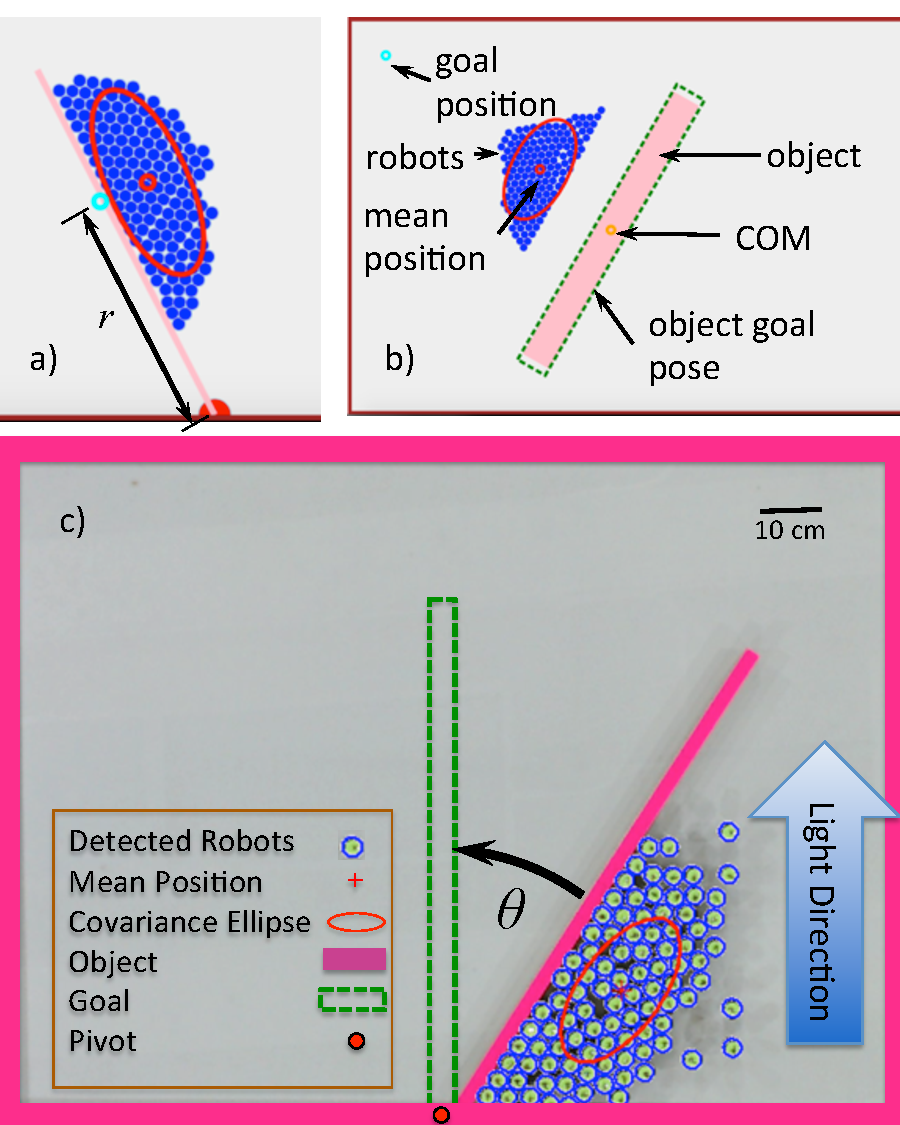
\includegraphics[width=.9\columnwidth]{CoverPhoto.pdf}
\end{center}
\vspace{-1em}
\caption{\label{fig:FirstImage}
%Torque control of an object is essential for manipulation unless objects are homogeneous discs, especially when there are narrow passageways or the objects must be aligned, e.g. sensors and emitters. 
%This paper provides the optimal position for a swarm to push to maximize torque production using a highly under-actuated system where all robots are controlled uniformly by the same input. 
(a) Simulation of robots exerting torque on a hinged ``door".
(b) Orientation control of a free long rod.
(c) Hardware robots applying torque to an object. See video attachment.% A full resolution video is available at \url{https://youtu.be/7Q5lu_ZFbxI}.
}
\vspace{-1em}
\end{figure}

With a single agent, torque control is straightforward: the agent simply maximizes the length of the movement arm to maximize torque. To make an agent push open a door, it should push on the edge furthest from the hinge. 
The optimal solution for a swarm of particles is not straightforward because they cannot all push at one position.

This chapter focuses on maximizing torque using the swarm's position distribution. 
Representative results are shown in Fig. \ref{fig:FirstImage}:  torque control using 56 mobile robots on a pivoted and a free object.




%%%%%%%%%%%%%%%
%%%%%%%%%%%%%%%

%%%%%%%%%%%%%%%%%%%%%%%%%%%%%%%%%%%%%%%%%%%%%%%%%%%%%%%%%%%
\section{Related work}\label{sec:RelatedWork}
%%%%%%%%%%%%%%%%%%%%%%%%%%%%%%%%%%%%%%%%%%%%%%%%%%%%%%%%%%%

Controlling the \emph{shape}, or relative positions, of a swarm of robots is a key ability for a range of applications.  Correspondingly, it has been studied from a control-theoretic perspective in  both centralized and decentralized approaches. For examples of each, see the centralized virtual leaders in \cite{egerstedt2001formation}, and the  gradient-based decentralized controllers  using control-Lyapunov functions in~\cite{hsieh2008decentralized}. However, these approaches assume a level of intelligence and autonomy in individual robots that exceeds the capabilities of many systems, including current micro- and nano-robots.  Current micro- and nano-robots, such as those in~\cite{Chowdhury2015,martel2015magnetotactic,Xiaohui2015magnetiteMicroswimmers} lack onboard computation.

This chapter focuses on centralized techniques that apply the same control input to both particles. 
Precision control requires breaking the symmetry caused by the uniform input.  
Symmetry can be broken using particles that respond differently to the uniform control signal, either through agent-agent reactions \cite{bertozzi2015ring}, or engineered inhomogeneity  \cite{Donald2013,bretl2007,beckerIJRR2014}. 
 The magnetic gradients of MRI scanners are \emph{uniform}, meaning the same force is applied everywhere in the workspace\cite{nosrati2018development}.
 This work assumes a uniform control with homogenous particles, as in~\cite{AaronManipulation2013}, and breaks the control symmetry using obstacles in the workspace. 

%The techniques in this paper are inspired by artificial force-fields. 

%\emph{Fluid-flow:} 
%Fluid flow along boundaries generates a shear force that pushes different parts of a body in opposing directions. 
%Most introductory fluid dynamics textbooks provide models~\citep{Munson2013}.
%Similarly, a swarm of robots under global control pushed along a boundary will experience shear forces.  
%This is a position-dependent force, and so can be exploited to control the configuration or shape of the swarm.  
% \citep{spears2006physics}~used these forces to disperse a swarm's spatial position for coverage for physics-based swarm simulations.

%\emph{Artificial Force-fields:}
%Much research has focused on generating non-uniform artificial force-fields that can be used to rearrange passive components. 
Alternative techniques rely on non-uniform inputs, such as artificial force-fields.
Applications have included techniques to design shear forces for sensorless manipulation of a single object by~\cite{lamiraux+2001:ra}.  
\cite{vose2012sliding} demonstrated a collection of 2D force fields generated by six degree-of-freedom vibration inputs to a rigid plate.  These force fields, including shear forces, could be used as a set of primitives for motion control to steer the formation of multiple objects. %However unlike the uniform control model in this paper, their control was multi-modal and position-dependent.
%\todo{talk about obstacles, think about adding goldberg}

%This paper develops control algorithms using uniform control fields, such as the magnetic resonance navigation \cite{nosrati2018development}.%field in a clinical MRI [insert a recent reference from Sylvain Martel using MRI].
Similarly, much recent work in magnet control has focused on exploiting inhomogeneities in the magnetic field to control multiple micro particles  using gradient-based pulling~\cite{Salmanipour2018EightDOF,Denasi2018independent}.  
Unfortunately, using large-scale external magnetic fields makes it challenging to independently control more than one microrobot unless the  distance between the electromagnetic coils is at the same length scales as the robot workspace~\cite{diller2016six, Denasi2018independent, Salmanipour2018EightDOF }. In contrast, % to methods that exploit inhomogeneities in the magnetic field to control multiple micro particles, e.g. \cite{Denasi2018independent}, that exploited nonlinearities generated by four magnetic coils in close proximity to the workspace to achieve trajectory control of two microspheres, 
 this chapter requires only a controllable constant gradient in orthogonal directions to position the particles.
% Systems like this one are poorly suited for PRM and RRT*-type methods\cite{lavalle2006planning} because if during a movement a collision occurs, that movement is irreversible.
   %Flow in a pipe or body lume

If a control input causes the particles to collide with obstacles at different times, inverting the control input does not undo the action. 
 Due to this lack of time-reversibility, techniques that require a bidirectional graph, e.g. PRM \cite{kavraki1996probabilistic} and RRT* \cite{lavalle2006planning} are not suitable.
  Instead, this chapter employs a greedy search strategy. 
%%%%%%%%%%%%%%%
%%%%%%%%%%%%%%%%%%%%%%%%%%%%%%%%%%%%%%%%%%%%%%%%%%%%%%%%%%%
%\section{Torque control}
%\label{sec:theory}
%%%%%%%%%%%%%%%%%%%%%%%%%%%%%%%%%%%%%%%%%%%%%%%%%%%%%%%%%%%
%\subsection{Controlling Torque}

%We derive inspiration from recent work on pulling with a swarm \cite{pulltogether}. The contribution of this work is to map swarm distributions to torque production.
%The orientation of an object's major axis is important when a swarm is manipulating a non-symmetric object through narrow corridors. 
%Orientation is controllable by applying torque to the object. 
%To change the output torque $\tau$ in~\eqref{eq:torque}, we can choose the direction and magnitude of the force applied $F$, and the moment arm from the object's center of mass (COM) $O$ to the point of contact $P$.
%We define a coordinate frame rooted at the COM, with the $x$-axis parallel to the object's longest axis. The resulting torque is:
%
%\begin{equation}
%\tau = F \times (P - O ).\label{eq:torque}
%\end{equation}
%
%We assume that the forces produced by individual particles add linearly. 
% As \cite{pulltogether} indicates, this is often a simplification of the true dynamics. 
% The swarm version of \eqref{eq:torque} is the summation of the forces contributed by $n$ individual particles:
%\begin{align}
%\tau_{\text{total}} &= \sum\limits_{i=1}^n \rho_i F_i \times (P_i - O ) \textrm{      and}   \label{eq:swarmtorque}\\
%F_{\text{total}} &= \sum\limits_{i=1}^n \rho_i F_i.  \label{eq:swarmforce}
%\end{align}
%Here $F_i$ is the force that the $i^{\textrm{th}}$ particle applies. 
%Not all particles are in contact with the object.  
%$\rho_i$ is an indicator variable: $\rho_i=1$ if the particle is in direct contact with the object or touching a chain of particle where at least one particle is in contact with the object. 
% Otherwise $\rho_i = 0$.
%The moment arm is the particle's position $P_i$ to the object's COM $O=[O_x,O_y]^{\top}$. 
% If all particles are identical and the control input is uniform, the force is equivalent for every particle and so $F_i $ equals some constant.
%

\section{Angle of repose}\label{sec:angle}




Consider a swarm of granular particles applying force to a rod. 
If the rod moves slower than the particles, these particles will build up behind the rod in a characteristic triangular shape defined by an apex angle. This piling up is common to all granular media, and the angle formed is a function of the \emph{angle of repose}. Three different values of angle of repose is shown in Fig.~\ref{fig:angle}. The center of mass of the rod is in the middle of the rod, but center of mass of the granular particles changes for different values of angle of repose. % for the media, see \cite{angleofRepose}. 
 By measuring the angle of repose for the particles shown in the top plot of Fig.~\ref{fig:AngleOfReposeForce}, we can estimate the force and torque that the swarm is applying to the rod as a function of the rod's length, the angle of repose, and orientation of the rod.
 We define the angle of repose as $\alpha$, the rod's orientation relative to 90$^\circ$ from the particle movement vector as $\theta$, and the rod's length as $\ell$. 
 \begin{figure}
\centering
\renewcommand{\figwid}{\columnwidth}
\begin{overpic}[width =\figwid]{Angle.pdf}%\put(1,55){a)}
\end{overpic}
\caption{\label{fig:angle} Different values of angle of repose is shown when granular particles move faster than the rod.
}
\end{figure}
By integrating over the triangular shape, the force applied to the rod (when a unit area of particles produces 1 N of force) is
\begin{figure}
\centering
\renewcommand{\figwid}{\columnwidth}
\begin{overpic}[width =0.6\figwid]{AngleOfRepose.pdf}%\put(1,55){a)}
\end{overpic}\\
\vspace{0.5em}
\begin{overpic}[width =0.6\figwid]{AngleOfReposeForce.pdf}%\put(1,55){a)}
\end{overpic}\\
\vspace{0.5em}
\begin{overpic}[width =0.6\figwid]{AngleOfReposeTorque.pdf}%\put(1,55){a)}
\end{overpic}
\vspace{-0.5em}
\caption{\label{fig:AngleOfReposeForce} Top plot shows colored particulate heaped up on pink-colored long rods. 
%Particulate is moving in the $-y$ direction, and the rods are tilted at $\theta=\{-45,-22.5,0,22.5,45\}^\circ$ with respect to the $x$ axis. 
% A thin gray line extends upwards from the rod COM, showing how more particulate is heaped on the right side of the rod for positive $\theta$ and more on the left side for negative $\theta$. 
%  This uneven particulate generates a restoring torque. 
 Middle plot shows the force applied to the rod and bottom the torque as a function of $\theta$ for four angle of repose values.
 %The rod length $\ell=1$. 
   The maximum torque values are shown with black dots.
% Generating code is in the attachment. 
%\vspace{-2em}
}
\end{figure}

\begin{align}
F(\theta,\alpha,\ell) =\left\{
\begin{array}{ll}
\frac{-\ell^2\Big(\cos(2\theta)-\cos(2\alpha)\Big)}{8\cos\alpha\sin{\theta}} &   -\alpha<\theta<\alpha\\
0 &    \textrm{otherwise .}\\
\end{array} 
\right .\\
\end{align}


%\begin{align}
%F(\theta,\alpha,l)  = \frac{l^2}{8\cos\alpha\sin{\theta}} \Big(\cos(2\theta)-\cos(2\alpha)\Big).
%\end{align}

The force for different angle of repose values are shown in the middle plot of Fig.~\ref{fig:AngleOfReposeForce}. 
Torque will also be similarly defined as
\begin{align}
\tau(\theta, \alpha, \ell) =\left\{
\begin{array}{ll}
\frac{\ell^3\Big(\cos(2\alpha)-\cos(2\theta)\Big)\sin{\theta} }{48\sin^2\alpha}&   -\alpha<\theta<\alpha\\
0 &    \textrm{otherwise .}\\
\end{array} 
\right.
\end{align}
Torque is shown in the bottom plot of Fig.~\ref{fig:AngleOfReposeForce}.
 Given sufficient particles to pile up to the angle of repose, this torque tends to stabilize the object to be perpendicular to the pushing direction.
Force is maximized with $\theta=0$, but the $\theta$ value that maximizes torque is a function of $\alpha$ and is defined as
\begin{align}
\theta_{t_{\max}} = \frac{\sin(\alpha)}{\sqrt{3}}.
\end{align}
To maximize the torque a particulate swarm applies on a thin rod, the swarm should move in the direction $-\theta_{t_{\max}} - 90^\circ$ with respect to the long axis of the rod.




%%%%%%%%%%%%%%%%%%%%%%%%%%%%%%%%%%%%%%%%%%%%%%%%%%%%%%%%%%%
\section{Covariance control}
\label{sec:covControl}
%%%%%%%%%%%%%%%%%%%%%%%%%%%%%%%%%%%%%%%%%%%%%%%%%%%%%%%%%%%
\begin{figure*}[!htb]
\begin{center}
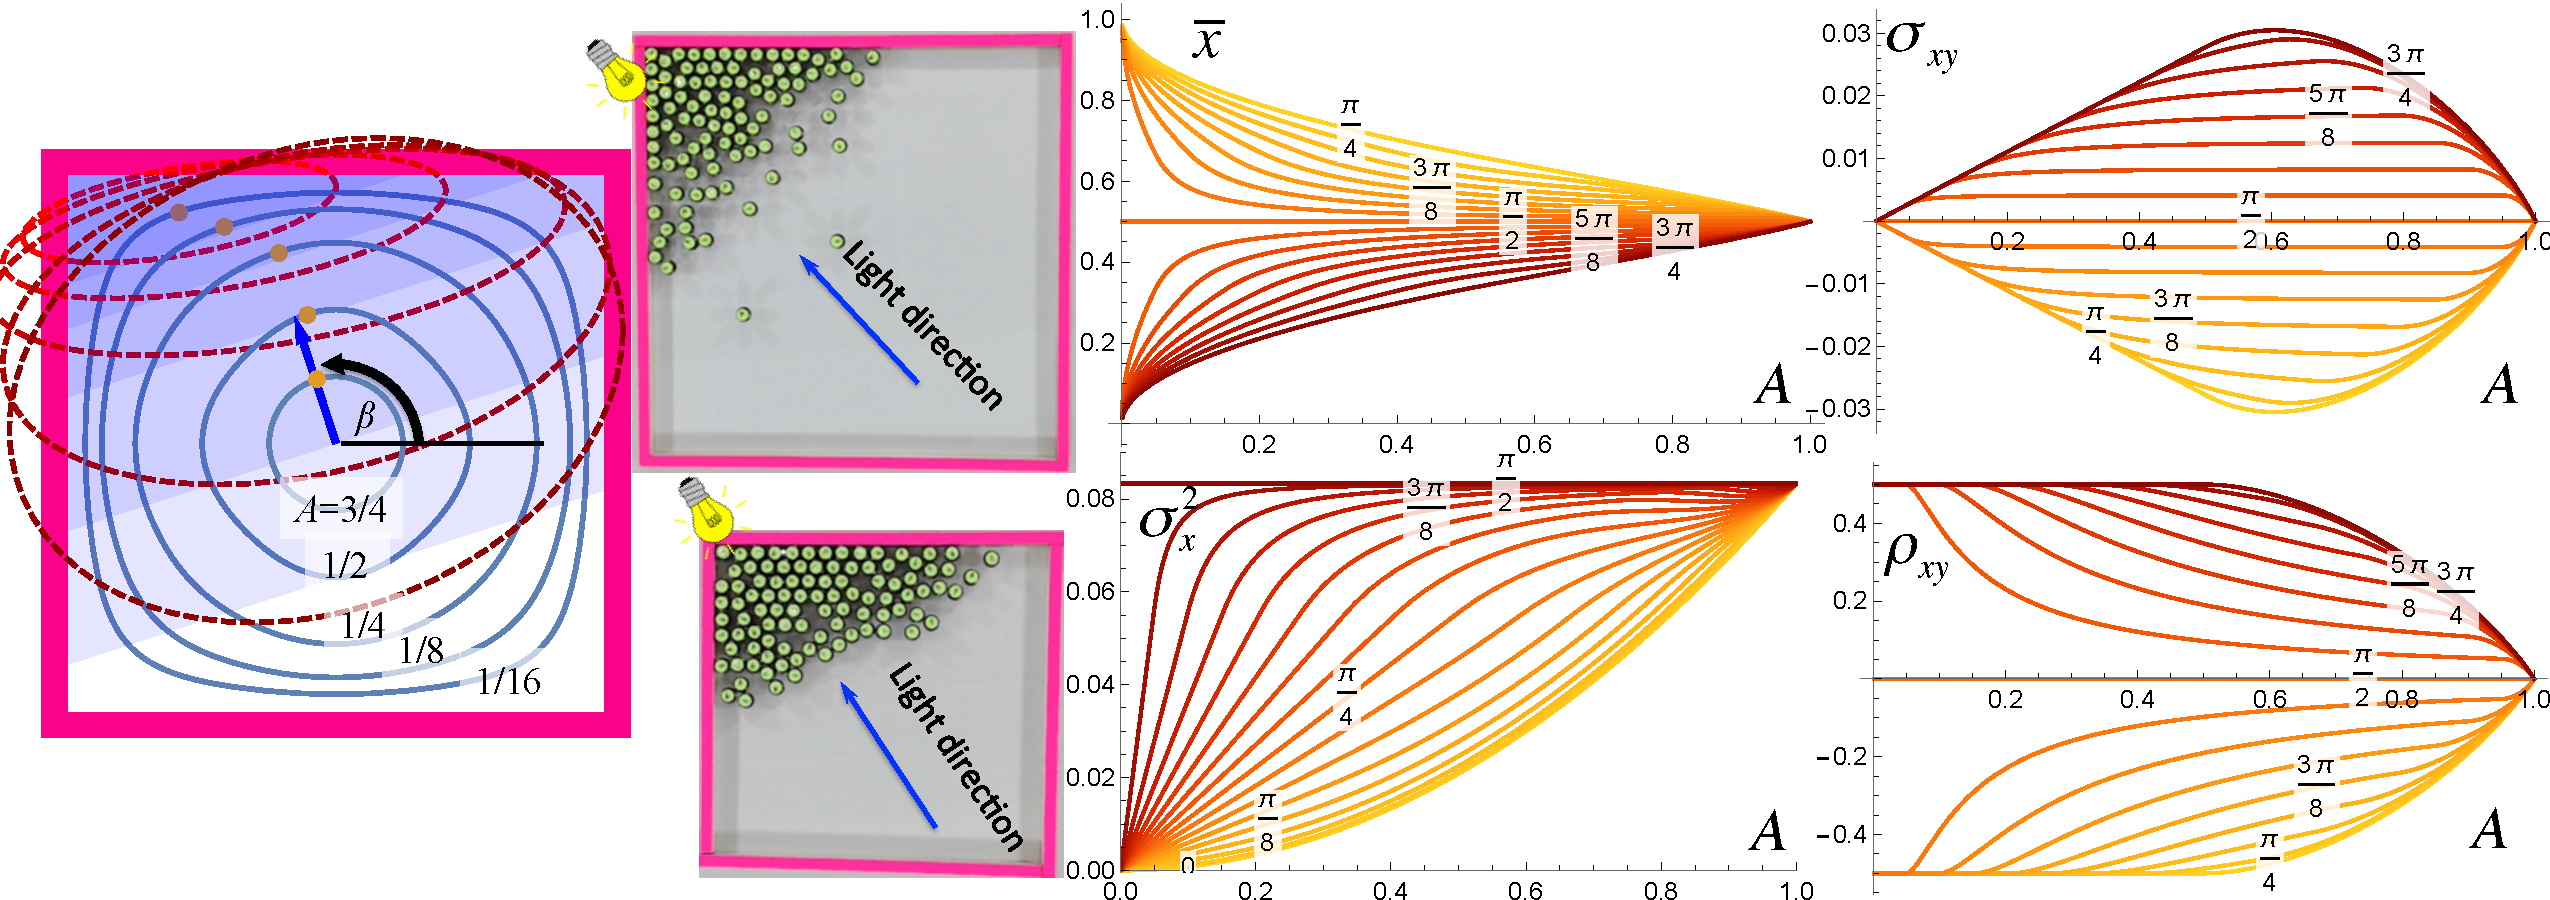
\includegraphics[width=\linewidth]{SquareFill.pdf} 
\vspace{-1em}
\caption{Pushing the swarm against a square boundary wall allows limited control of the shape of the swarm, as a function of swarm area $A$ and the commanded movement direction $\beta$. Left plot shows locus of possible mean positions for five values of $A$.  %The locus morphs from a square to a circle as $A$ increases.  The covariance ellipse for each $A$ is shown with a dashed line.
 Center shows two corresponding arrangements of kilobots. % At right is $\bar{x}(A), \sigma_{xy}(A), \sigma_x^2(A),$ and $\rho(A)$ for a range of $\beta$ values. See online interactive demonstration at \cite{Zhao2016mathematicaSquare}.
 }
\label{fig:SquareFill}
\end{center}
\end{figure*} 
\begin{figure*}[!htb]
\begin{center}
\vspace{-1em}
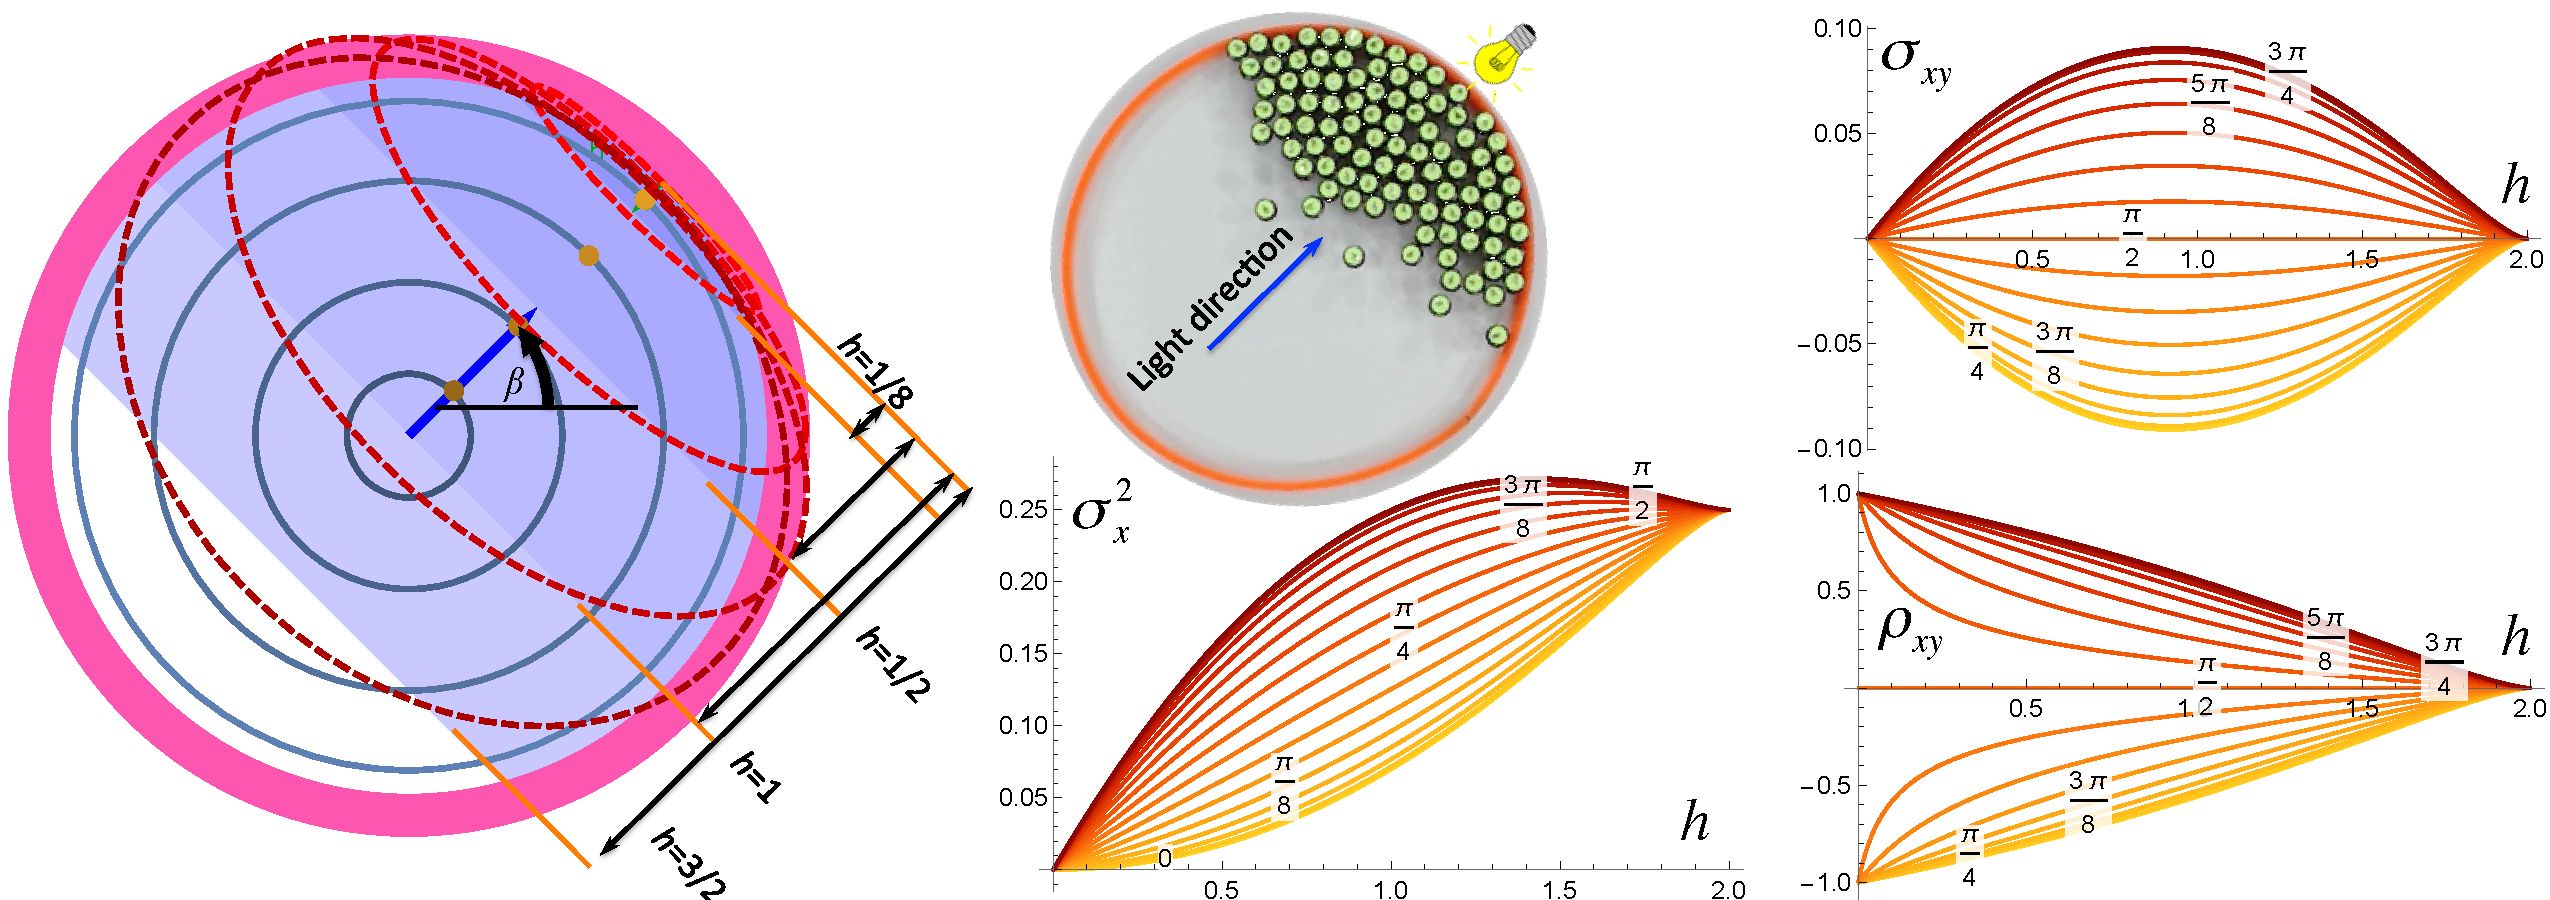
\includegraphics[width=\linewidth]{CircleFill.pdf} 
\vspace{-1em}
\caption{Pushing the swarm against a circular boundary wall allows limited control of the shape of the swarm, as a function of the fill level $h$ and the commanded movement direction $\beta$. Left plot shows locus of possible mean positions for four values of $h$. %The locus of possible mean positions are concentric circles. %See online interactive demonstration at \cite{Zhao2016mathematica}.
}  
\label{fig:CircleFill}
\end{center}
\vspace{-1em}
\end{figure*} 
Covariance control as well as mean position and variance control is needed when the swarm is moving through narrow passageways. This section discusses ideas to control covariance of the swarm using boundaries.

\subsection{Using boundaries: stable configurations of a swarm}\label{subsec:FluidInTank}
One method to control a swarm's shape in a bounded workspace is to simply push in a given direction until the swarm conforms to the boundary. Like fluid settling in a tank, the stable final configuration minimizes potential energy.
\paragraph{Square workspace}
%The formulas for means $(\bar{x},\bar{y})$, covariance $(\sigma^2_x,\sigma^2_y,\sigma_{xy})$, and correlation $\rho_{xy}$ are as follows: 
We first examine the mean $(\bar{x},\bar{y})$, covariance $(\sigma^2_x,\sigma^2_y,\sigma_{xy})$, and correlation $\rho_{xy}$ of a large swarm of robots as they move inside a square workspace under the influence of a force pulling in the direction $\beta$. The swarm is large, but the robots are small in comparison, and together occupy a constant area $A$, $A\in [0,1]$. Under a global input, the swarm moves to a side of the workspace and forms a polygonal shape that minimizes potential energy, as shown in Fig.~\ref{fig:SquareFill},  see also \cite{Zhao2016mathematicaSquare}.

The range for the global input angle $\beta $ is [0,2$\pi $). In this range, the swarm assumes eight different polygonal shapes. 
These shapes alternate between triangles and trapezoids when the area $A$$<$1/2, and between squares with one corner removed and trapezoids when $A$$>$1/2.

Computing means, variances, covariance, and correlation requires integrating over $R$, the region containing the swarm:  %This is simplified using an indicator function $\bm{1}_A(x,y)$ that returns 1 if inside the region containing the swarm, and 0 else. 
%The formulas for means $(\bar{x},\bar{y})$, covariance $(\sigma^2_x,\sigma^2_y,\sigma_{xy})$, and correlation $\rho_{xy}$ are as follows: %, integrated over the unit square with $x$ and $y$ from 0 to 1:

\begin{align}
\bar{x} &=\frac{\iint_R x \,dx\,dy}{A} \label{eq:meanInSquareWorkspace}
\text{, }\qquad \bar{y}=\frac{\iint_R y \,dx\,dy}{A} \text{, }\\
%\end{align}
%\begin{align}
\sigma^2_x &=\frac{\iint_R \left(x-\bar{x}\right)^2  \,dx \,dy}{A}  \label{eq:varInSquareWorkspace}
\text{, } \sigma^2_y =\frac{\iint_R  \left(y-\bar{y}\right)^2 \,dx \,dy}{A}\text{, and}\\
%\end{align}
%\begin{align}
\sigma_{xy} &= \frac{\iint_R  \left(x-\bar{x}\right) \left(y-\bar{y}\right) \, dx \,dy}{A} \label{eq:covAndcorrInSquareWorkspace}
\text{, }\rho_{xy} = \frac{\sigma^2_x}{\sigma_x\sigma_y}.
\end{align}

The region of integration $R$ is the polygon containing the swarm. For example, if $A<1/2$ and the force angle is $\beta$, the mean when $R$ is a triangular region in the lower-left corner is:
\begin{align}\label{eq:meanInSquareWorkspaceLL}
\bar{x}(A,\beta) &= \frac{\int_0^{\sqrt{2 A \tan (\beta)}} \left(\int_0^{\cot (\beta) \left(\sqrt{2 A \tan (\beta)}-x\right)} \, dy\right) x \, dx}{A} \nonumber \\
	&=\frac{ \sqrt{2}}{3} \sqrt{A \tan (\beta )}\\
\bar{y}(A,\beta) &= \frac{\int_0^{\sqrt{2 A \tan (\beta)}} \left(\int_0^{\cot (\beta) \left(\sqrt{2 A \tan (\beta)}-x\right)} y \, dy\right) \, dx}{A} \nonumber\\
	&=\frac{\sqrt{2}}{3}  \sqrt{A \cot (\beta )}.
\end{align}
The full equations are included in the appendix~\cite{2016arXiv160901830S}, and are summarized in Fig.~\ref{fig:SquareFill}. A few highlights are that the correlation is maximized $\pm$1/2 when the swarm is in a triangular shape. The covariance of a triangle is always $\pm(A/18)$. Variance is minimized in the direction of $\beta$ and maximized orthogonal to $\beta$ when the swarm is in a rectangular shape. The range of mean positions are maximized when $A$ is small.

%%%%%%%%%%%%%%%%%%%%%%%%%%%%%%%
\paragraph{Circular workspace}
Though rectangular boundaries are common in artificial workspaces, biological workspaces are usually rounded.
Similar calculations can be made for a circular workspace.  The workspace is a circle centered at (0,0) with radius 1 and thus area $\pi$.
For notational simplicity, the swarm is parameterized by the global control input signal $\beta$ and the fill-level $h$.  
Under a global input, the robot swarm fills the region under a chord with area
\begin{align}
A(h) = \arccos(1-h)-(1-h) \sqrt{(2-h) h}.
\end{align}
For a circular workspace, the locus of mean positions are aligned with $\beta$ and the mean position is at radius $r(h)$ from the center:
\begin{align}
r(h) = \frac{2 (-(h-2) h)^{3/2}}{3 \left(\sqrt{-(h-2) h} (h-1)+\arccos(1-h)\right)}.
\end{align}
Variance $\sigma^2_x(\beta,h)$ is maximized at $\beta = \pi/2+n \pi$ and $h\approx1.43$, while covariance is maximized at $\beta = \pi3/4+n \pi$ and $h\approx0.92.$ For small $h$ values, correlation approaches $\pm1$. Results are displayed in Fig.~\ref{fig:CircleFill}, see also \cite{Zhao2016mathematica}.

%Smashing the swarm to the corner walls will cause some correlation between \emph{x} and \emph{y} axes. Eq. ~\ref{eq:Wall} shows the relation between number of robots and area provided and the correlation we can reach with it.
%%TODO: ADD the equation for showing the correlation Vs area, vs number of robots
% This equation shows that we are not able to reach high correlations bigger than $|0.5|$. Fig. ~\ref{fig:wallCorrelation} shows the different mean positions and correlations we are able to reach. There are ways and corridors that the swarm needs to pass and also to keep the majority of it. If we use the wall corners technique and the way needs a very high correlation to pass, a remarkable number of the swarm members will be lost, and we may lose track of them due to their small size. Meanwhile, the variance of the swarm would get bigger and bigger that it would not anymore be able to deliver sufficient payloads. For this reason we have thought another idea which uses \emph{friction} to make correlations.
%


\subsection{Using boundaries: friction and boundary layers}\label{subsec:WallFriction}
Global inputs move a swarm uniformly.  
Shape control requires breaking this uniform symmetry.  
A swarm inside an axis-aligned rectangular workspace can reduce variance normal to a wall by simply pushing the swarm into the boundary. 
If the swarm can flow around each other, pushing the swarm into a boundary produces the limited set of configurations presented in Sec.~\ref{subsec:FluidInTank}.
%Controlling covariance by pushing the swarm into a boundary requires changes to the boundary.  
%An obstacle in the lower-right corner is enough to generate positive covariance, but generating both positive and negative covariance requires additional obstacles.  
%Requiring a special obstacle configuration also makes shape control dependent on the local environment. 
Instead of pushing our robots directly into a wall, the following sections examine an oblique approach  using boundaries that generate friction with the robots. 
 These frictional forces are  sufficient to break the symmetry caused by uniform inputs.  
Robots touching a wall have a friction force that opposes movement along the boundary.  
This causes robots along the boundary to move more slowly than robots in free-space. 
  
Let the control input be a vector force $\vec{F}$ with magnitude $F$ and orientation $\theta$ with respect to a line perpendicular to and into the nearest boundary. $N$ is the normal or perpendicular force between the robot and the boundary. The force of friction $F_f$ is nonzero if the robot is in contact with the boundary and  $\sin(\theta) < 0$. The resulting net force on the robot, $F_{\text{\emph{forward}}}$, is aligned with the wall and given by
\begin{align}
F_{\text{\emph{forward}}} &=  F \sin(\theta) - F_f  \nonumber \\
\text{where }  F_f &= \begin{cases}  \mu_f N, &  \mu_f N < F \sin(\theta)  \label{eq:frictionmodel}  \\
F \sin(\theta), & \text{else} \end{cases} \\ %\sign(F \sin(\theta) ) \cdot  \max(0, | F sin\theta |- |F_f|)
\text{and } N &= F \cos(\theta) .\nonumber
\end{align}
 Fig.~\ref{fig:friction} shows the resultant forces on two robots when one is touching a wall. 
Though each receives the same inputs,  they experience different net forces.
  For ease of analysis, the following algorithms assume $\mu_f$ is infinite and robots touching the wall are prevented from sliding along the wall.
This means that if one robot is touching the wall and another robot is free, the touching robot will not move when the control input is parallel or into the wall. 
There are many alternate models of friction that also break control symmetry. Fig.~\ref{fig:friction}c shows fluid flow along a boundary.  Fluid in the free-flow region moves uniformly, but flow decreases to zero in the boundary layer \cite{fluidMechanics}.  Force in such a system can be calculated as
\begin{align}
%u(y) = u_0 \left(1- \frac{(y-h)^2}{h^2}\right) = u_0 \frac{y}{h} \left(2- \frac{y}{h}\right) \label{eq:boundarylayerflow} THiS EQUATION IS TERRIBLE! PLOT IT.
F_{forward}(y) &= F - F_f\begin{cases}  \frac{h-y}{h}   , &  y<h \label{eq:boundarylayerflow} \\
0, & \text{else} \end{cases}.
\end{align}

The next section shows how a system in a rectangularly bounded workspace with friction model \eqref{eq:frictionmodel} can arbitrarily position two robots. 
\begin{figure}[h]
\begin{center}
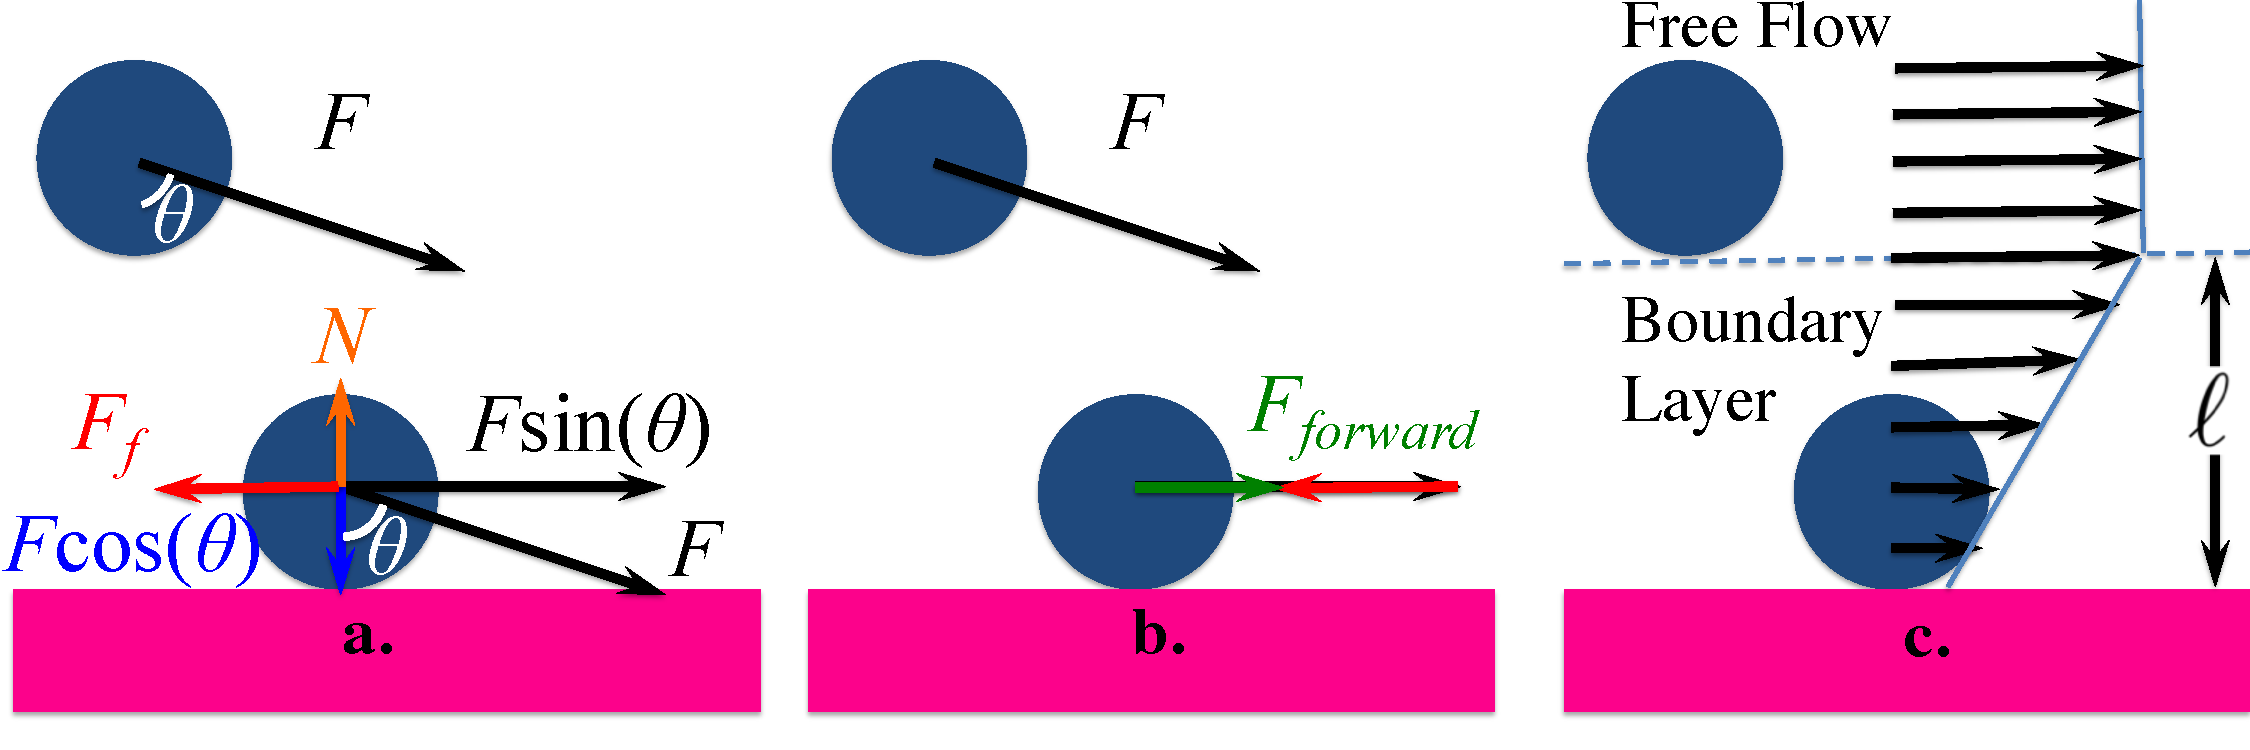
\includegraphics[width=0.8\columnwidth]{friction.pdf} 
\vspace{-1em}
\caption{(a,b) Wall friction reduces the force for going forward $F_{\text{\emph{forward}}}$ on a robot near a wall, but not for a free robot. (c) velocity of a fluid reduces to zero at the boundary.
\label{fig:friction}
}\vspace{-1em}
\end{center}
\end{figure} 




\subsection{Maximizing correlation using wall friction}\label{subsec:ClosedLoopCovarianceControl}
Using the environment to individually move $n$ particles to goal positions in Alg. \ref{alg:PosControlNRobots} requires $O(n^2)$ time, while  Alg. \ref{alg:optimalAlg} can only control two particles. The controllers in Section \ref{sec:theory} are efficient because they require only a single move but the range of possible configurations are limited. This section presents an efficient technique to generate desired correlations.

Assume an obstacle-free, bounded, unit-size, square workspace. 
 As shown in Fig.~\ref{fig:SquareFill}, the maximum correlation occurs when the swarm is pushed in the direction $\beta = 3\pi/4$. 
 This correlation as a function of swarm area $A$ is never larger than 1/2, and the maximum correlation decays to 0 as $A$ grows to 1. By  \eqref{eq:covAndcorrInSquareWorkspace}, this maximum correlation is:
\begin{align} \label{eq:GravityCorrelation}
\rho_{xy} =  \begin{cases}  \frac{1}{2}  , &  0\le A\le \frac{1}{2}  \\
% \frac{3 A (2 (A-2) A+1)}{4 A \left(A^2+3 \sqrt{2-2 A}-6\right)-12 \sqrt{2-2 A}+17}-1
 \frac{3 A (2 (A-2) A+1)}{4 A^3-24 A+\sqrt{2} (12 A-12) \sqrt{1-A}+17}-1
 , & \frac{1}{2} \le A\le 1
\end{cases}.
\end{align}
 If friction obeys the linear boundary layer model of \eqref{eq:boundarylayerflow} with boundary layer thickness $h$ and maximum friction $F_f$ equal to the maximum applied force $F$, we can generate  larger correlations.
 If the swarm size is smaller than $\approx 0.43$ and the boundary layer is sufficiently thick we can generate correlations larger than 1/2  using boundary friction.

 Assume that the swarm is initialized in the lower-left corner, in a rectangle of width $w$ and height $A/w$. 
 Such a rectangular configuration can be accomplished using the variance controllers from \cite{ShahrokhiIROS2015}. 
  If the swarm is then commanded to move a distance $L$ to the right, components of the swarm outside the boundary friction layer of height $h$ move further than components near the boundary. 
   The swarm is contained in a region $R$ composed of no more than three stacked components: at bottom a parallelogram inclined to the right top, at middle a rectangle, and at top a parallelogram inclined to the left top. These regions can be defined by the rectangle's left side, bottom, and top:
\begin{align}
r_{\text{left}} &= \min (L,1-w),\nonumber \\
r_{\text{bottom}} &=\min \left(\frac{A}{w}, h\frac{r_{\text{left}}}{L}  \right) \text{and}\nonumber \\
r_{\text{top}}  &= \min \left(\frac{A}{w}, 1-h\frac{r_{\text{left}}}{L}  \right).
\end{align}
If $\frac{A}{w} \le r_{\text{top}}$ the top parallelogram has no area. 
 Similarly, if $r_{\text{top}} \le r_{\text{bottom}}$ the rectangle has no area. 
The mean, variance, and correlation are calculated  using \eqref{eq:meanInSquareWorkspace}, \eqref{eq:varInSquareWorkspace}, and \eqref{eq:covAndcorrInSquareWorkspace} over the region $R$:
\begin{align} \iint_R f(x,y) \, dx \,dy &=  \int_0^{r_{\text{bottom}}}  \int_{\frac{L}{h}y}^{\frac{L}{h}y+w}  f(x,y)  dx \, dy \label{eq:correlationFriction} \\
&+\int_{r_{\text{bottom}}}^{r_{\text{top}}} \int_{r_{\text{left}}}^{r_{\text{left}} +w} f(x,y)    dx \, dy \nonumber\\
&+\int_{r_{\text{top}}}^{\frac{A}{w}} \int_{-\frac{L (y-r_{\text{top}})}{h}+r_{\text{left}}}^{r_{\text{left}}+w-\frac{L (y-r_{\text{top}})}{h}} f(x,y)   dx \, dy .\nonumber
\end{align}
 
 Given an environment parameterized by $A$ and $h$, efficient correlation control consists of choosing the $w,L$ pair  that generates the desired positive correlation.
  Negative correlations can be generated by initializing the swarm in the upper left, or lower right.

\subsection{Efficient control of correlation}
%A set of simulations were conducted to demonstrate the importance of boundary friction.  
This section examines maximum correlation values as a function of  $w,L$ using \eqref{eq:correlationFriction}
from Section  \ref{subsec:ClosedLoopCovarianceControl}. 
The maximum correlation using boundary layer friction $\displaystyle  \max_{w,L} \left( \rho(A,h,w,L) \right)$ can be found by gradient descent, as shown in Fig.~\ref{fig:ControlledCorrelation}. 
For swarms with small area, this method enables generating the full range of correlations $\pm 1$, while the stable configuration method from Section \ref{sec:theory} could only generate correlations $\pm 1/2$.  As  the swarm area $A$ increases above $\approx 0.43$, the stable configuration method is more effective.
Larger boundary layers $h$ enable more control of correlation.
The multimedia attachment shows efficient control of correlation with simulations using the 2D physics engine Box2D~\cite{catto2010box2d} and 144 disc-shaped robots with boundary layer model \eqref{eq:boundarylayerflow}.



\begin{figure}
\begin{center}
	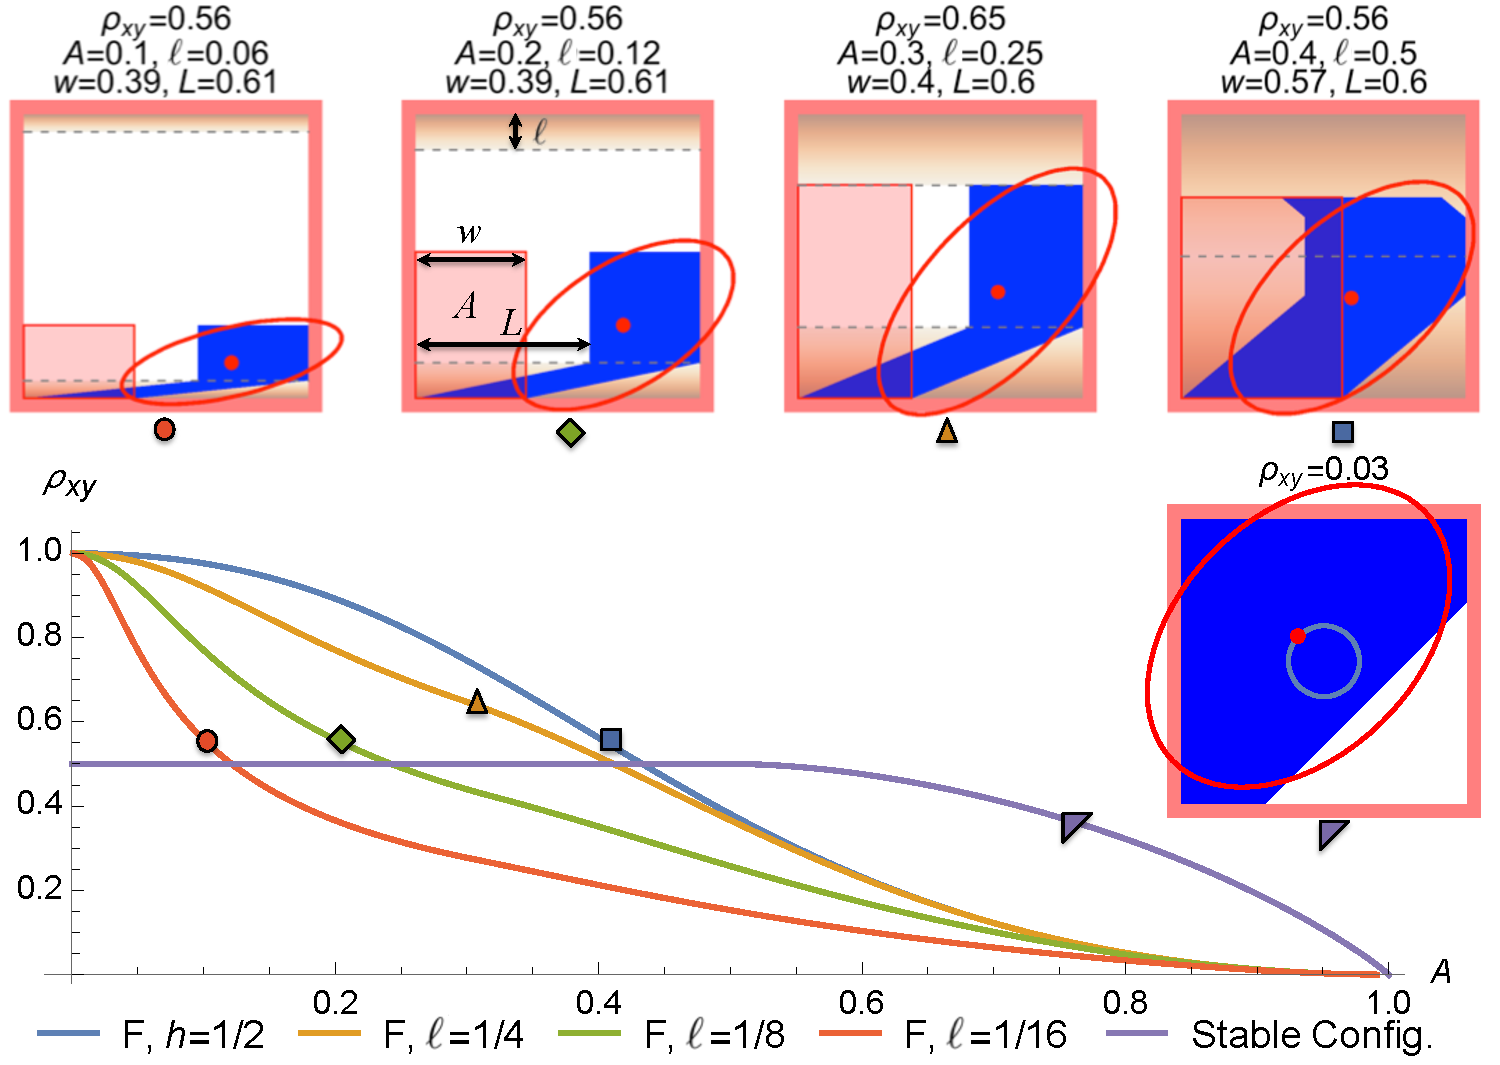
\includegraphics[width=\columnwidth]{ControlledCorrelation.pdf}
\end{center}
\vspace{-1em}
\caption{\label{fig:ControlledCorrelation}
Analytical results comparing maximum correlation $\rho_{xy}$ under the boundary layer friction model of \eqref{eq:correlationFriction} with four boundary layer thicknesses $h$ and the stable triangular configuration \eqref{eq:GravityCorrelation}.
}\vspace{-1em}
\end{figure}
\subsection{Hardware experiment: control of covariance}
To demonstrate covariance control, up to 100 kilobots were placed on the workspace and manually steered with lights, using friction with the boundary walls to vary the covariance from  -4000 to 3000 cm$^2$.  The resulting covariance is plotted in Fig.~\ref{fig:covExperiment}, along with snapshots of the swarm.




\begin{figure}
\begin{center}
	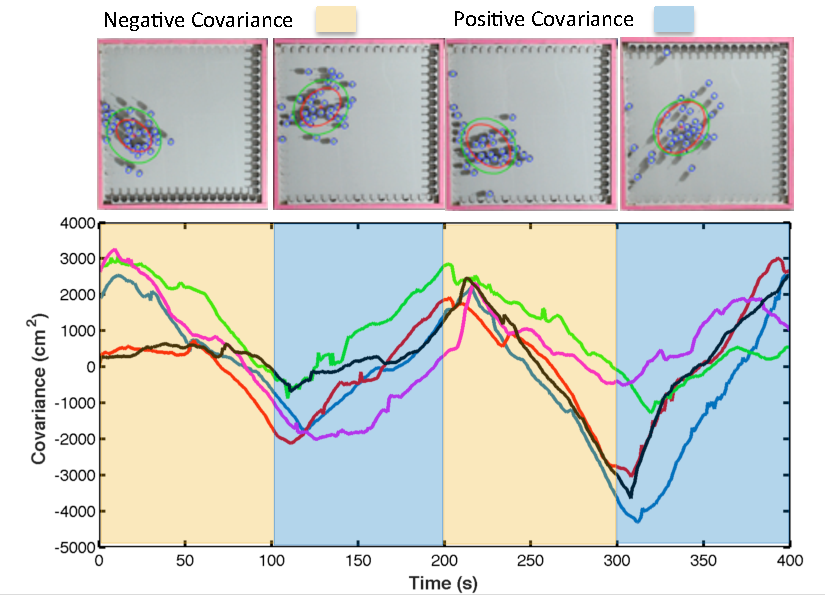
\includegraphics[width=\columnwidth]{newExperiment.pdf}
\end{center}
%\vspace{-1em}
\caption{\label{fig:covExperiment}
Hardware demonstration steering $\approx 50$ kilobot robots to desired covariance. The goal covariance is negative in first 100 seconds and is positive in the next 100 seconds. The actual covariance is shown in different trials. Frames above the plot show output from machine vision system and an overlaid covariance ellipse.
%\vspace{-2.5 em}
}
\end{figure}


%

\section{Position control of $n$ robots using boundary interaction}\label{sec:PostionControlnRobots}
%%%%%%%%%%%%%%%%%%%%%%%%%%%%%%%%%%%%%%%%%%%
The ideas from Alg. \ref{alg:optimalAlg}  can be extended to control the position of $n$ particles using walls with non-slip contact.
The solution is complete, but not optimal, and requires the starting and final configurations of particles to be disjoint.
The solution described here is an iterative procedure with $n$ loops. 
 The $k^{\text{th}}$ loop moves the $k^{\text{th}}$ robot from a \emph{staging zone} to the desired position in a \emph{build zone}. 
  All robots move according to the uniform input, but due to non-slip wall contacts, at the end of the $k^{\text{th}}$ loop, robots 1 through $k$ are in their desired final configuration in the build zone, and robots $k+1$ to $n$ are in the staging zone. 
   See Fig.~\ref{fig:simulationNrobot} for a schematic of the build and staging zones.

\begin{figure}
\begin{center}
	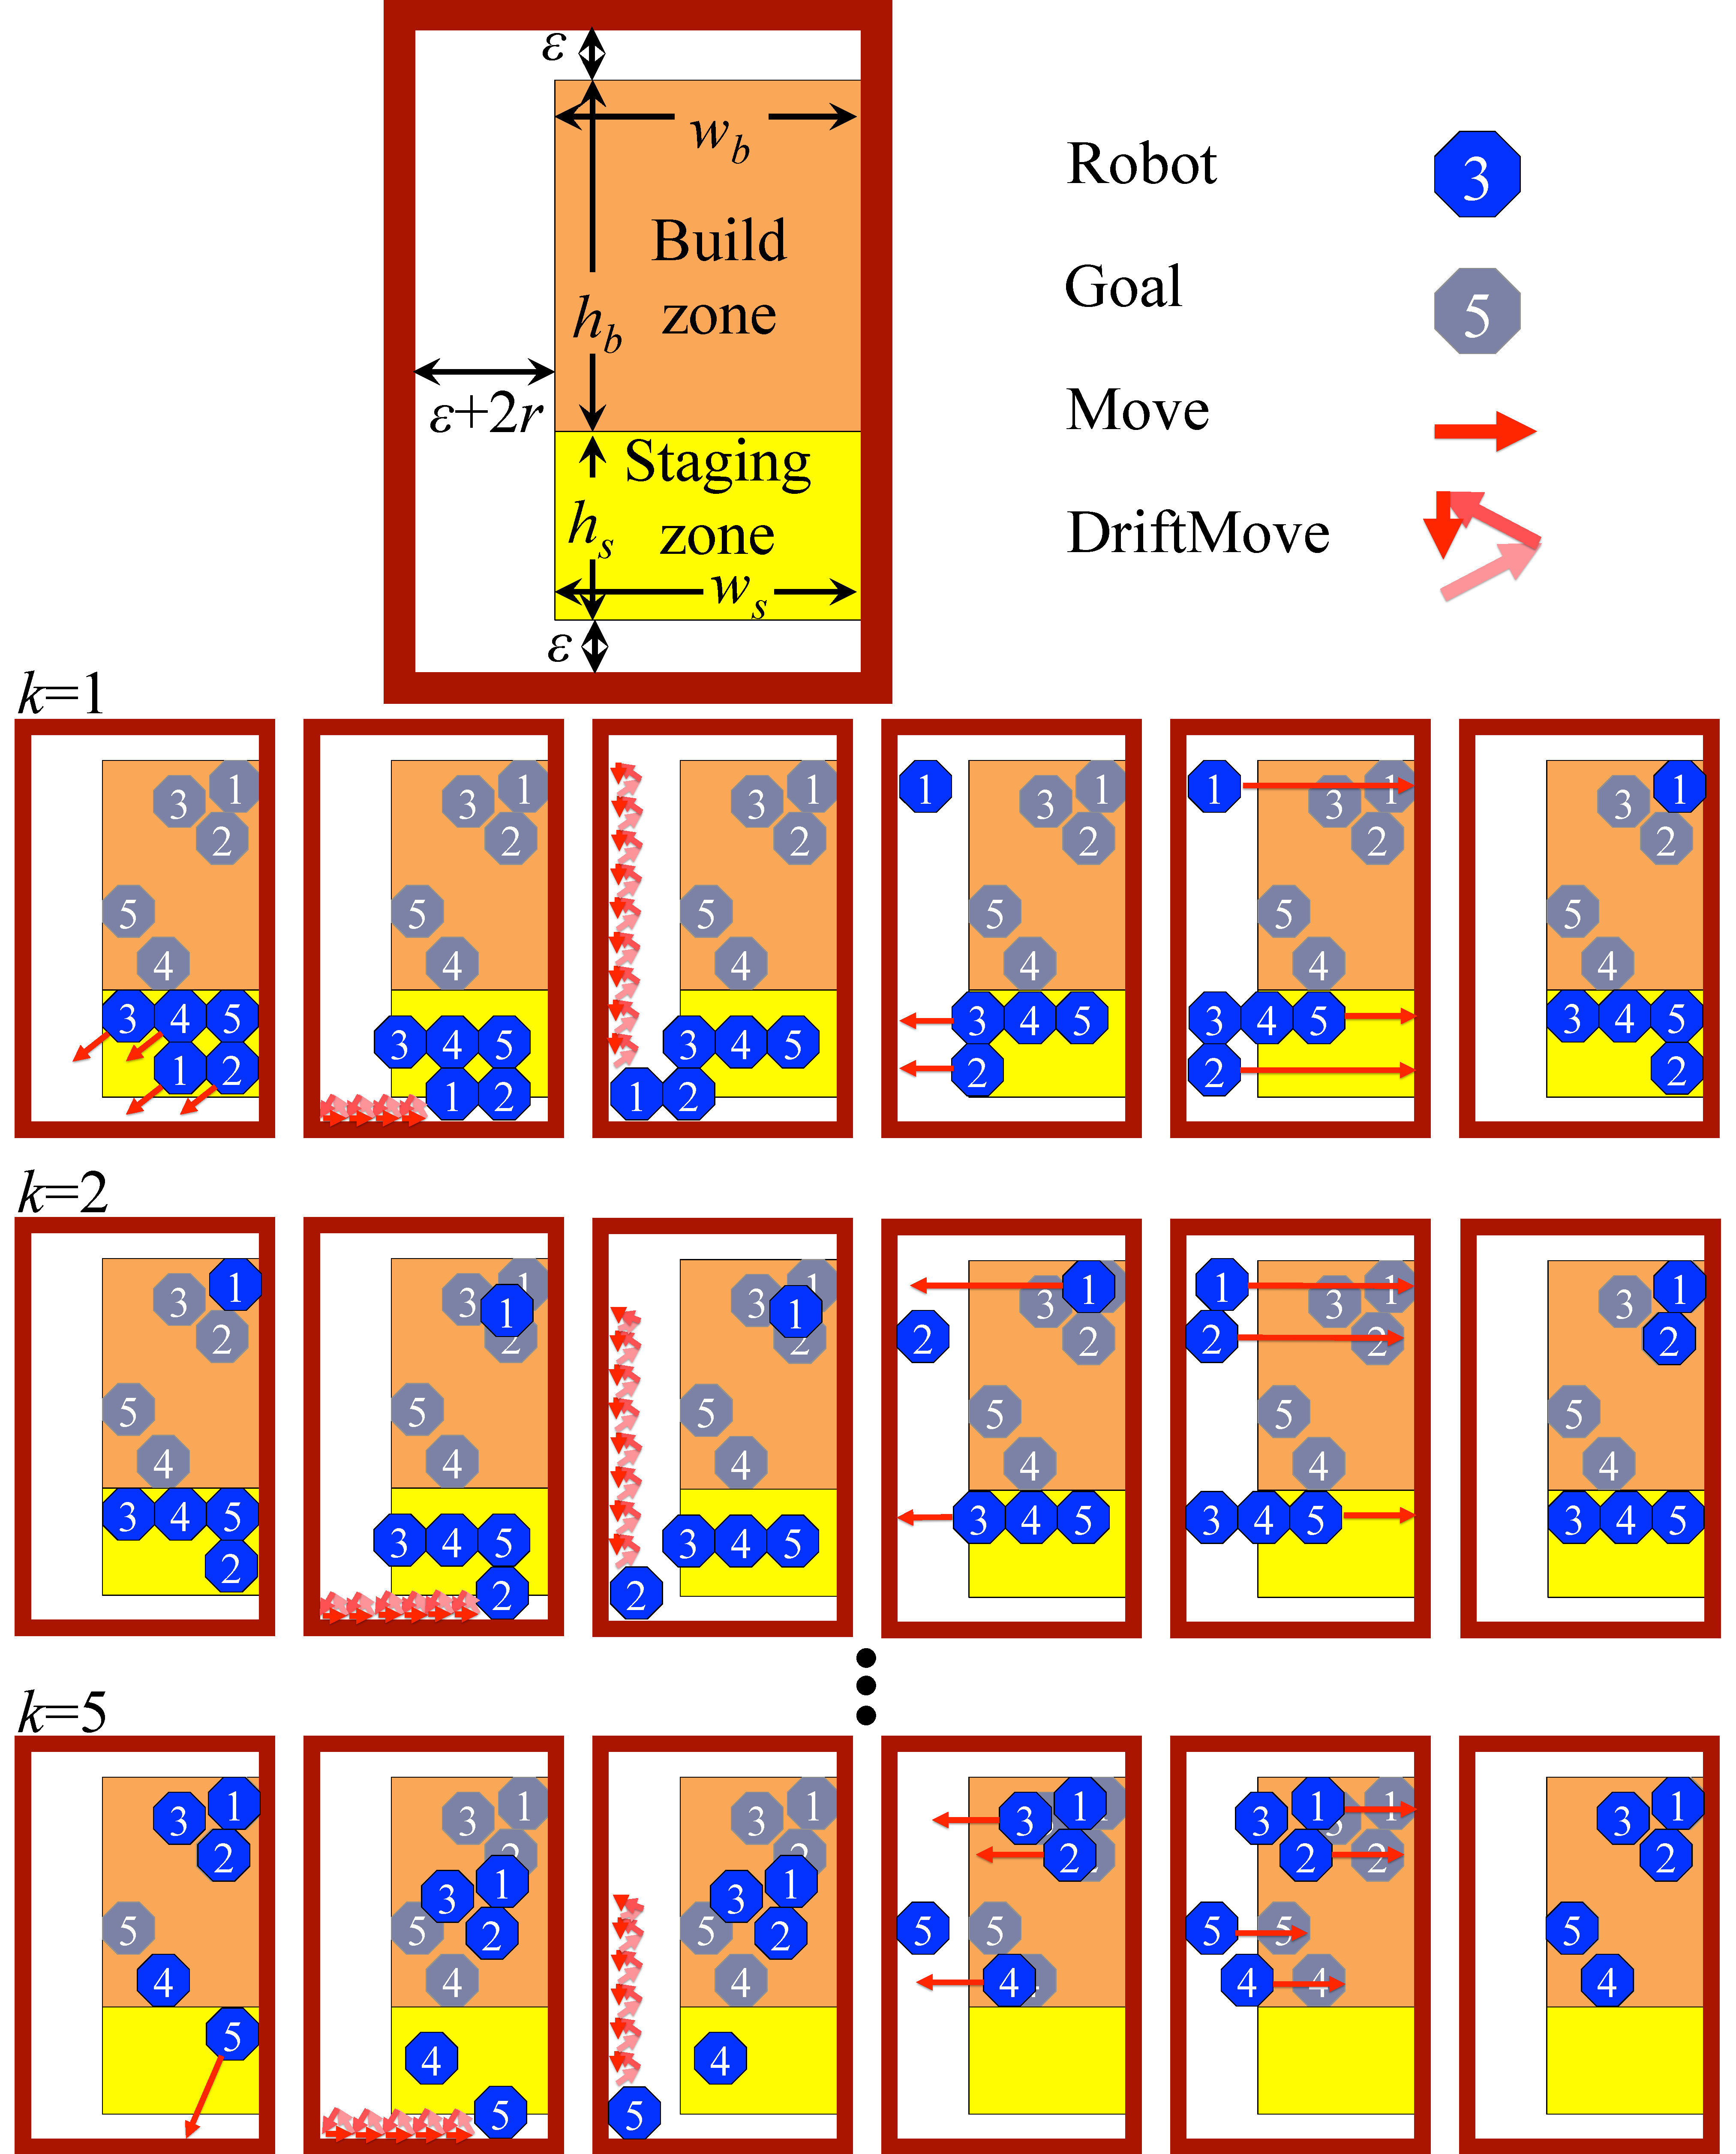
\includegraphics[width=1.0\columnwidth]{PositionNrobots.pdf}
\end{center}
\vspace{-1em}
\caption{\label{fig:simulationNrobot}
Illustration of Alg.\ \ref{alg:PosControlNRobots}, $n$ robot position control  using walls with non-slip contact.
}
\end{figure}

Assume an open workspace with four axis-aligned walls with non-slip contact.
The axis-aligned build zone of dimension $(w_b, h_b)$ containing the final configuration of $n$ robots must be disjoint from the axis-aligned staging zone of dimension $(w_s, h_s)$  containing the starting configuration of $n$ robots.
 Without loss of generality, assume the build zone  is above the staging zone.  Let $d$ be the diameter of the particles.
Furthermore, there must be at least $\epsilon$ space above the build zone, $\epsilon$ below the staging zone, and $\epsilon + d$ to the left of the build and staging zone.  The minimum workspace is then $(\epsilon + d + \max(w_b,w_s), 2\epsilon + h_s,h_b)$.

The $n$ robots position control algorithm relies on a $\text{\sc DriftMove}(\alpha, \beta, \epsilon,\theta)$ control input, described in Alg.~\ref{alg:DriftMove} and shown in Fig.\  \ref{fig:driftmove}.
For $\theta = 0^\circ$, a drift move consists of repeating a triangular movement sequence $\{ (\beta/2,-\epsilon),(\beta/2,\epsilon),(-\alpha,0)\}$. 
 Any particle touching a top wall moves right $\beta$ units, while every particle not touching the top moves right $\beta-\alpha$.

\begin{figure}
\begin{center}
%
\includegraphics[width=.47\columnwidth]{driftmove0.pdf}
%	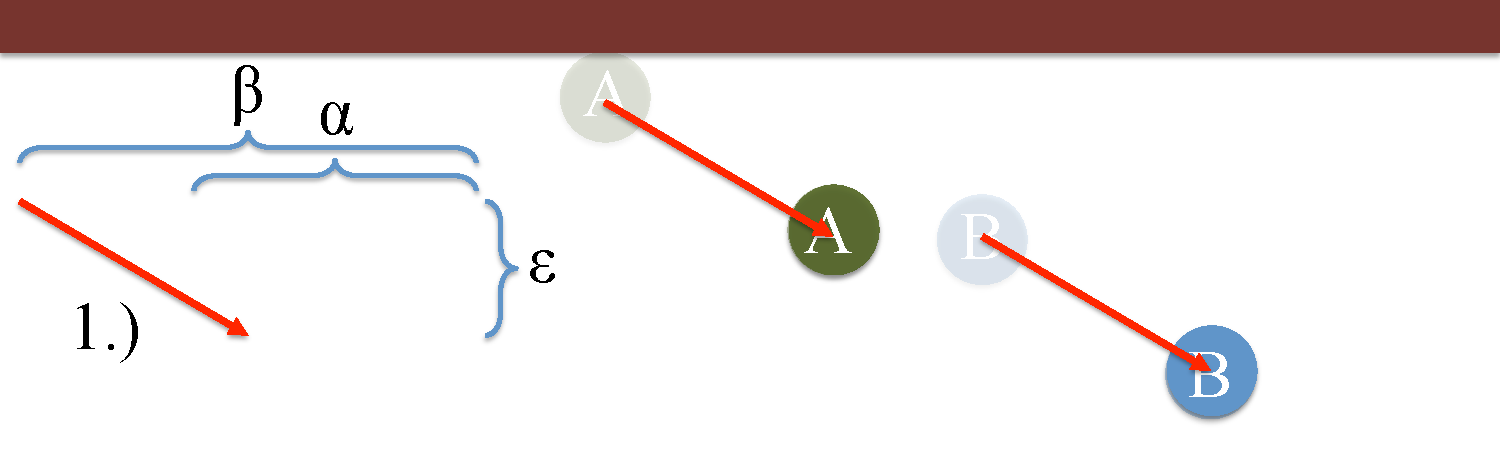
\includegraphics[width=.47\columnwidth]{driftmove1.pdf}
%	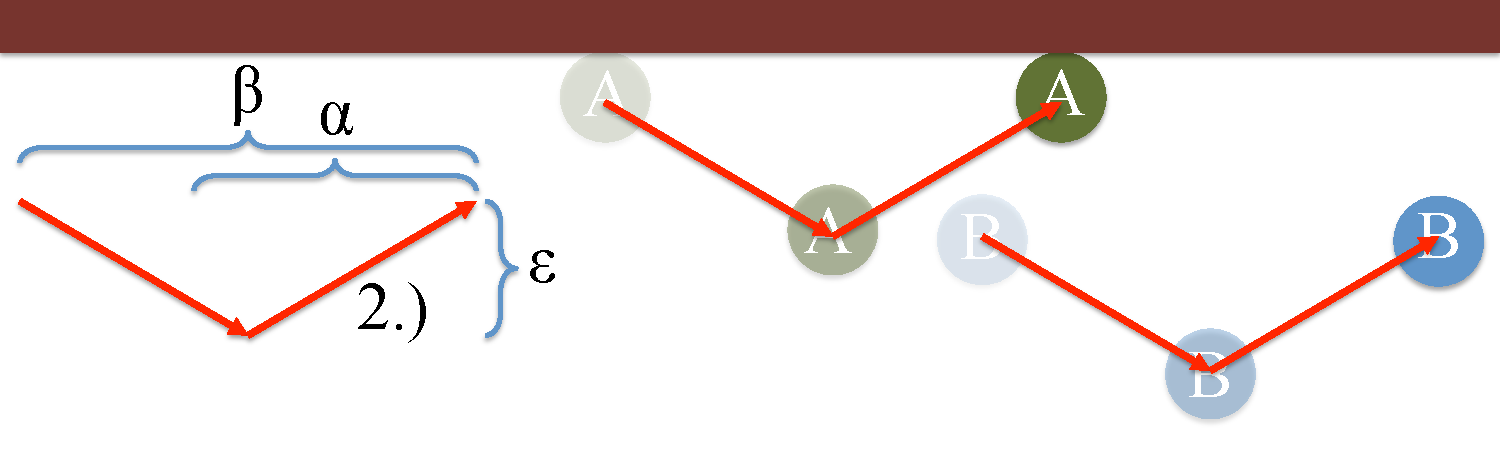
\includegraphics[width=.47\columnwidth]{driftmove2.pdf}
	\includegraphics[width=\columnwidth]{driftmovefullres.pdf}
\end{center}
\vspace{-1em}
\caption{\label{fig:driftmove}
A  $\text{\sc DriftMove}(\alpha, \beta, \epsilon,0^\circ)$ repeats a triangular movement sequence $\{ (\beta/2,-\epsilon)$, $(\beta/2,\epsilon)$, $(-\alpha,0)\}$. At the sequence end, robot $A$ has moved $\beta$ units right, and robot $B$ has moved $\beta-\alpha$ units right.}
\vspace{-1em}
\end{figure}

Let $(0,0)$ be the lower left corner of the workspace, $p_k$ the $x,y$ position of the $k^{\text{th}}$ robot, and $f_k$ the final $x,y$ position of the $k^{\text{th}}$ robot. Label the robots in the staging zone from left-to-right and bottom-to-top, and the $f_k$ configurations top-to-bottom and right-to-left as shown in Fig.~\ref{fig:construction2d}.

\begin{algorithm}
\caption{PositionControl$n$Robots($k$)}\label{alg:PosControlNRobots}
\begin{algorithmic}[1]
\State Move( $-\epsilon, d/2-p_{ky}$) % move  away from right wall and down till robot k touches bottom


\While{ $p_{kx} > d/2$} 
\State $\text{\sc DriftMove}(\epsilon, \min(p_{kx} - d/2,\epsilon), \epsilon,180^\circ)$    %drift move left until kth robot touches left wall
\EndWhile

\State $m \gets \operatorname{ceil}(\frac{f_{ky}-d/2}{\epsilon})$
\State $\beta \gets \frac{f_{ky}-d/2}{m}$
\State $\alpha \gets \beta - \frac{d/2 - p_{ky}-\epsilon}{m}$
\For{ $m$ iterations}
\State $\text{\sc DriftMove}(\alpha, \beta, \epsilon,90^\circ)$    %move kth robot to f_{ky} and leave the rest in position.
\EndFor

\State Move ($d/2+\epsilon-f_{kx}, 0$)  % move the group to the left until k is in the correct relative x position
\State Move ($f_{kx}-d/2, 0$)  

\end{algorithmic}
\end{algorithm}


\begin{algorithm}
\caption{ {\sc DriftMove}($\alpha,\beta,\epsilon,\theta$)
}\label{alg:DriftMove}
particles touching the wall move $\beta$ units, while particles not touching the wall move $\beta-\alpha$ units.
\begin{algorithmic}[1]
\State $R = \begin{bmatrix} \cos(\theta) & -\sin(\theta) \\
 \sin(\theta) & \cos(\theta)  \end{bmatrix}$
\State {\sc Move}$(R \cdot [\beta/2,-\epsilon]^\top)$ 
\State  {\sc Move}$(R \cdot [\beta/2,\epsilon]^\top)$ 
\State  {\sc Move}$(R \cdot [-\alpha,0]^\top)$ 
\end{algorithmic}
\end{algorithm}


Alg. \ref{alg:PosControlNRobots} proceeds as follows:  
First, the robots are moved left away from the right wall, and down so all robots in $k^{\text{th}}$ row touch the bottom wall.
Second, a set of $\operatorname{DriftMove}$s are executed that move all robots in $k^{\text{th}}$ row left until $k$ touches the left wall, with no net movement of the other robots.
Third, a set of $\operatorname{DriftMove}$s are executed that move only robot $k$ to its target height and return the other robots to their initial heights. 
Fourth, all robots except robot $k$ are pushed left until robot $k$ is in the correct relative $x$ position compared to robots 1 to $k-1$.
Finally, all robots are moved right until robot $k$ is in the desired target position. Running time is $O(n(w+h))$.



The hardware platform depicted in Fig.~\ref{fig:construction2d} is an assembled practical setup that assumes that $\epsilon= 1$ cm. 
The workspace is a $7\times 7$ cm grid space. 
All particles are 3D-printed plastic whose top is a 1cm diameter cylinder with a narrower base that encapsulates a steel bearing ball.
Non-slip wall contact is generated by a toothed wall design to keep particles from moving out of place while implementing the drift move. 
The workspace boundary is mounted on top of a white sheet of cardboard.
Underneath the cardboard, a grid of 3mm diameter magnets glued with 1 cm spacing to a thin board generates the uniform control input.
 A video attachment  shows the algorithm at work. 
This discretized setup requires several modifications to Alg.~\ref{alg:PosControlNRobots}.
 In this demonstration, all moves are 1 cm in length.
   All drift moves are a counterclockwise \emph{square} move  of size 1 cm$\times$1 cm. 
   Once the $k^{\text{th}}$ particle gets to its designated location in each loop, a correction step is implemented. 
   This correction step increases by two the total number of moves required per particle.
   Fig.~\ref{fig:simulationNrobot} shows there are only 6 stages per particle involved in Alg.~\ref{alg:PosControlNRobots}.
The fixed step algorithm requires 8 stages per particle as shown in Fig.~\ref{fig:construction2d}. 

A significant difference between Alg.~\ref{alg:PosControlNRobots} and the fixed move implementation of it is that Alg.~\ref{alg:PosControlNRobots}
enables placing particles at arbitrary, non-overlapping locations, while the fixed move implementation requires goal locations at the center of grid cells. 

\begin{figure}
\begin{center}
	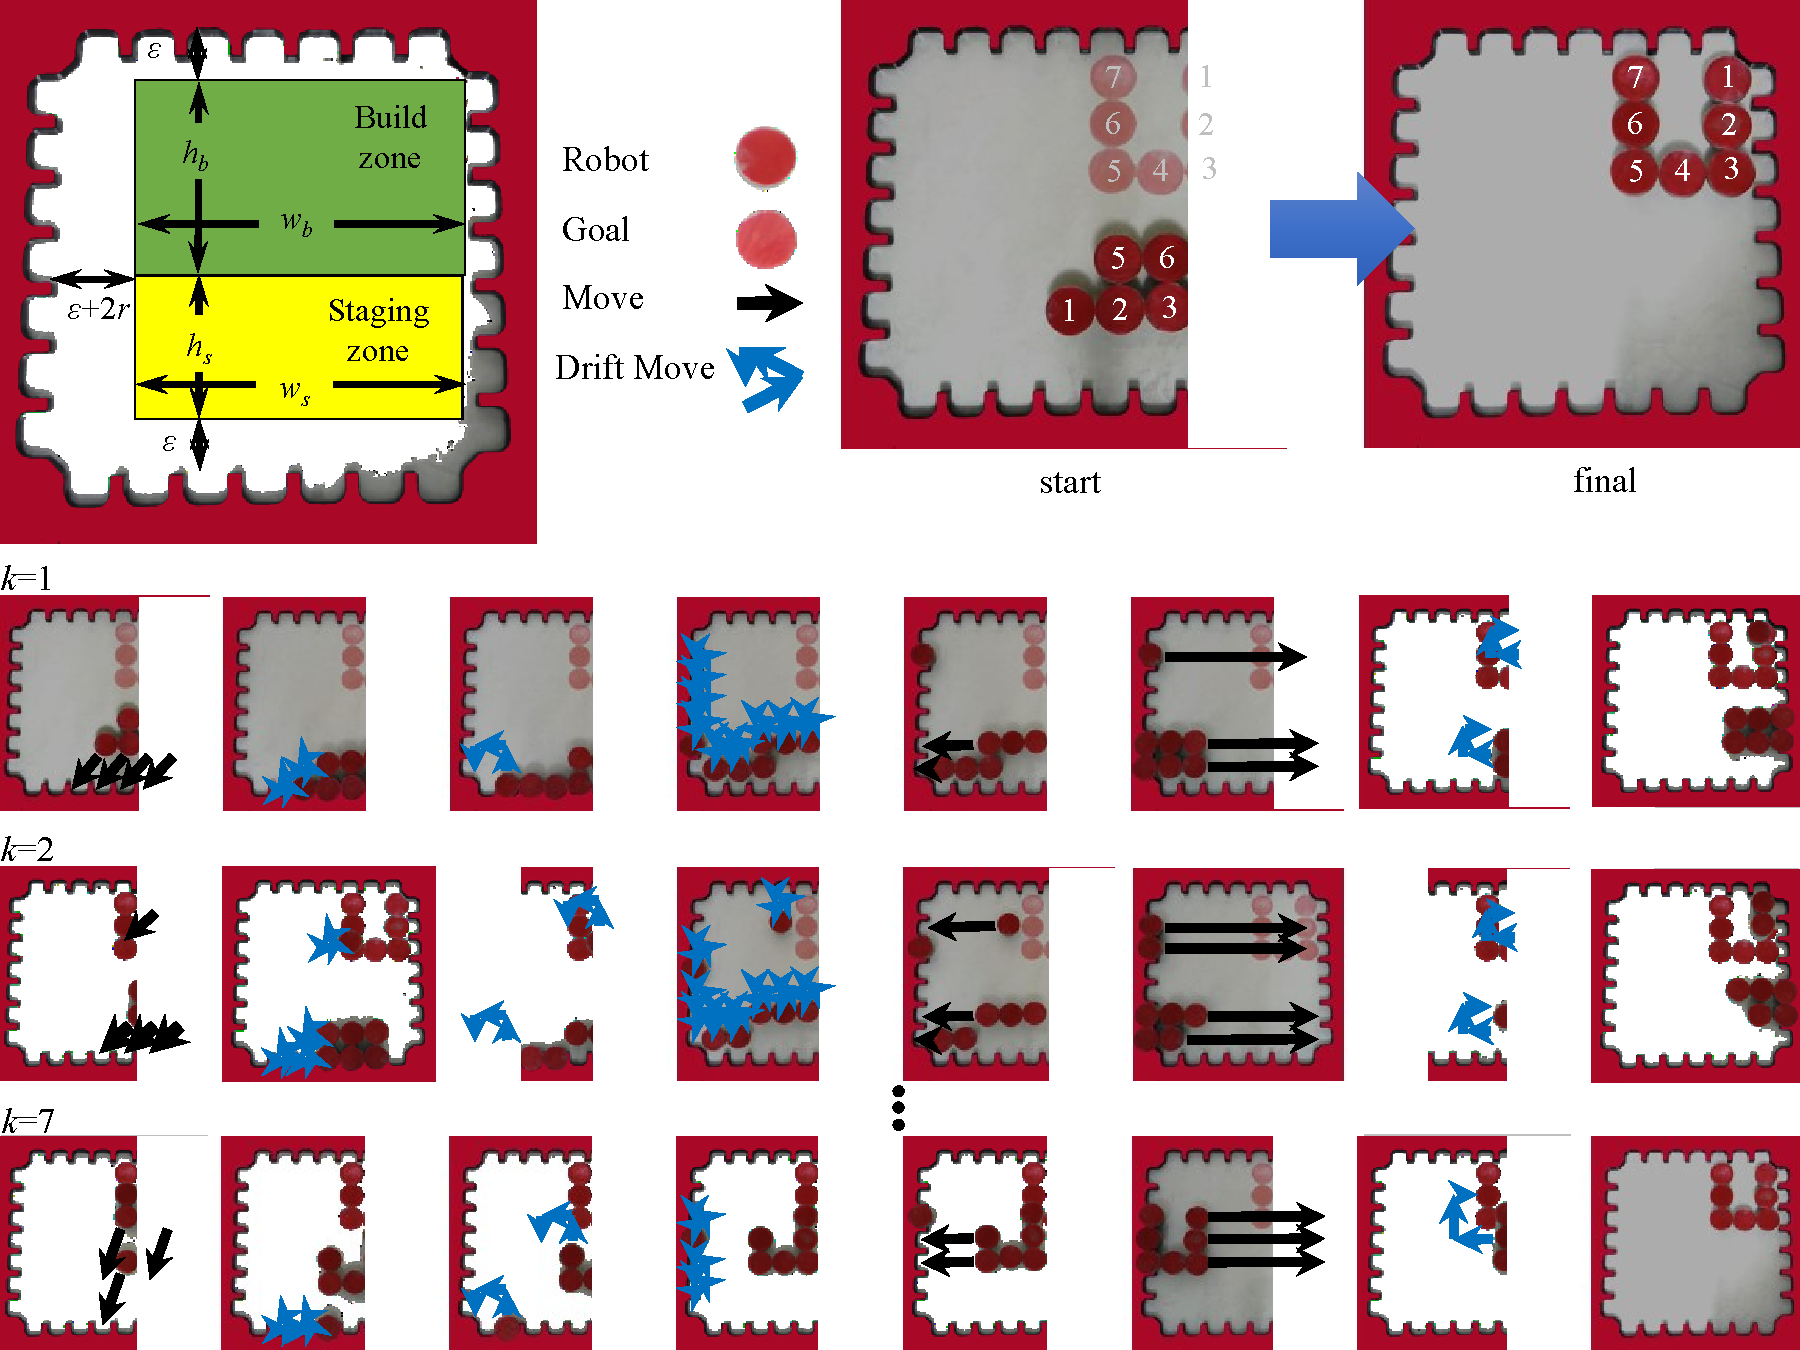
\includegraphics[width=1.0\columnwidth]{multirobotSliderHardware2.pdf}
\end{center}
\vspace{-1em}
\caption{\label{fig:construction2d}
Illustration of Alg.\ \ref{alg:PosControlNRobots}, discretized $n$ robot position control  using walls that enforce non-slip contact.
}
\end{figure}


%%%%%%%%%%%%%%%
%%%%%%%%%%%%%%%
%
\section{Simulation}\label{sec:simulation}


%Two simulations were implemented using non-slip contact walls for position control.  The first controls the position of two robots, the second controls the position of $n$ robots.  

%\subsection{Position Control of Two Robots}
\begin{figure}
\centering
\begin{overpic}[width=0.49\columnwidth]{worstnum.pdf}\put(0,75){a)}\end{overpic}
\begin{overpic}[width=0.49\columnwidth]{worstdist.pdf}\put(0,75){b)}\end{overpic}
\begin{overpic}[width=0.49\columnwidth]{middlegoalnum.pdf}\put(0,75){c)}\end{overpic}
\begin{overpic}[width=0.49\columnwidth]{middlegoaldist.pdf}\put(0,75){d)}\end{overpic}
\caption{\label{fig:contour}
Plots show performance with one goal on the boundary.
}
\end{figure}

\begin{figure}
\centering
%\begin{overpic}[width=\columnwidth]{deltanum.pdf}\end{overpic}\\
%\vspace{1em}
\begin{overpic}[width=\columnwidth]{deltadist.pdf}\end{overpic}
\vspace{-1em}
\caption{\label{fig:deltanumdist}
The worst case path length occurs when particles must swap antipodes. This can never be achieved but can be asymptotically approached. Plot shows decreasing error as the number of moves grows.
} 
\end{figure}


\begin{figure}
\centering
\renewcommand{\figwid}{1\columnwidth}
{
\begin{overpic}[width =\figwid]{contourDistnew.png}\put(-2,10){\begin{turn}{90} \tiny{unique particles}
\end{turn}}

\end{overpic}
\vspace{1em}
\begin{overpic}[width =\figwid]{JustSimulationV6.png}\put(-2,10){\begin{turn}{90} \tiny{unique particles}
\end{turn}}

\end{overpic}
\begin{overpic}[width =\figwid]{identical.png}\put(-2,6){\begin{turn}{90} \tiny{interchangeable particles}
\end{turn}}
\end{overpic}
}\caption{\label{fig:contourPlots}{Starting positions of particles $1$ and $2$ and goal position of particle $2$ are fixed, and $\epsilon=0.001$.
 The top row of contour plots show the distance if robot $1$'s goal position is varied in $x$ and $y$. The bottom row shows the number of moves required for the same configurations.}
\vspace{-1em}
}
\end{figure}
Algorithm \ref{alg:optimalAlg}  was implemented in Mathematica using particles with zero radius. 
%An online interactive demonstration and source code of the algorithm are available at \cite{Shahrokhi2015mathematicaParticle}.
%  Fig.~\ref{fig:shapeControlMathematica1}  shows  an implementation of this algorithm with robot initial positions represented by hollow squares and final positions by circles. 
 %Dashed lines show the shortest route if robots could be controlled independently, while solid lines show the optimal shortest  path using uniform inputs.
 
 The contour plots in Fig.~\ref{fig:contour} left show the length of the path for two different settings. Top row considers \{$s_1,s_2,g_1$\} = \{$(0.2,0.2),(-0.1,-0.1),(-0.2,0)$\} and bottom row considers  \{$s_1,s_2,g_1$\} = \{$(0.2,0.2),(-0.1,-0.1),(0,0)$\} in a workspace with $r= 0.5$, and $g_2$ ranging over all the workspace. Fig.~\ref{fig:contour} right shows the total distance of the path. This plot shows the nonlinear nature of the path planning. The path length grows when the goals have $\pi$ difference and are very close to the boundary. TODO:???? We need to discuss the new plots.
 The worst case occurs when the ending points are at antipodes along the boundary ($\pi$ angular distance). This can never be achieved but can be asymptotically approached as shown in Fig.~\ref{fig:deltanumdist}. 
 Fig.~\ref{fig:contourPlots} shows the same concepts in a square workspace. Fig.~\ref{fig:contourPlots} top and middle row considers the particles for three arbitrary starting and goal positions for the particles. All of the discussed plots have considered the particles to be unique. If particles are interchangeable and it does not matter to put the specific particle to its goal location, the path length will be significantly smaller. The bottom row of  Fig.~\ref{fig:contourPlots} considers interchangeable particles with the same configuration as the middle row with unique particles.
 
 %If the length of each side of the square workspace is $L$, the worst case path length is $(\sqrt{2}+2)L$.
 
% The plots in Fig.~\ref{fig:deltanumdist} show the exponentially increasing number of moves and distance when the accuracy of reaching to the goal ($\delta$) is getting to zero when the goal positions have $\pi$ difference with each on the boundaries.











%%%%%%%%%%%%%%%
%%%%%%%%%%%%%%%
%%%%%%%%%%%%%%%%%%%%%%%%%%%%%%%%%%%%%%%%%%%%%%%%%%%%%%%%%%%%
\section{Experimental Results}\label{sec:expResults}
%%%%%%%%%%%%%%%%%%%%%%%%%%%%%%%%%%%%%%%%%%%%%%%%%%%%%%%%%%%
\begin{figure*}[htb!]\label{fig:3dPrinted}
\centering
\vspace{1.5em}
%\begin{overpic}[width=\columnwidth]{firstImage.jpg}\end{overpic}
\begin{overpic}[width=2\columnwidth]{3dexperiment.pdf}\end{overpic}
\\
\vspace{1em}
\begin{overpic}[width=2\columnwidth]{realTripe.pdf}\end{overpic}
\caption{\label{fig:story}
Frames showing particle positions before and after control inputs. Top row: small intestine phantom. Bottom row: cow stomach tissue.
} \vspace{-1em}
\end{figure*}

To demonstrate Alg.~\ref{alg:optimalAlg} experimentally, we performed several tests.
Each used the same magnetic setup shown in Fig.~\ref{fig:IntroPic}.
% The figure might need to be referenced 
 Two different intestine models were employed, the first a 3D-printed cross-section representation of a small intestine, and the second a cross-section of a bovine stomach.
 
 \subsection{Magnetic Manipulation Setup}
 
 The magnetic manipulation system has two pairs of electromagnetic coils, each with iron cores at their centers, and arranged orthogonal to each other. The iron core at the center of each coil concentrates the magnetic field towards the workspace. An Arduino and four SyRen regenerative motor drivers were used for control inputs to the coils. Finally, a FOculus F0134SB 659 x 494 pixel camera was attached to the top of the system, focusing on the workspace which was backlit by a $\SI{15}{\watt}$ LED light strip. 
 
To obtain experimental data, the test samples (the phantom intestine model and the bovine cross section) were placed in laser-cut acrylic discs and then immersed in corn syrup. Corn syrup was used to increase the viscosity to 12000 cP for the experiments. Spherical $\SI{1}{\milli\metre}$ magnets (supermagnetman \#SP0100-50) were used as our particles. Our experimental setup did not perfectly implement the system dynamics in \eqref{eq:swarmDynamicsAndFric}. In particular, the magnetic field in this setup is only approximately uniform. The magnetic force varies in both magnitude and orientation. As shown in the video attachment, this non-uniformity causes the particle closer to the coil to move faster than the other particle. This phenomenon makes it easier to increase particle separation than to decrease separation, but this can be compensated because boundary collisions easily decrease the separation. Also, magnetic forces are not exactly parallel, but point toward the center of the activated coil. Algorithm~\ref{alg:optimalAlg} still works despite these non-uniformities, but sometimes requires additional iterations.
 
%explain the magnetic field strength used, the camera system (briefly)
%explain the particles used

%explain the fluid used in the model.

\subsection{Intestine Phantom Model}

The intestine phantom model was used first and was made to mimic the geometry of an intestine and its villi. The model consists of a circular ring with an outer diameter of $\SI{50}{\milli\metre}$, an inner diameter of $\SI{46}{\milli\metre}$, and 60 $\SI{2}{\milli\metre}$ long protrusions on its inner surface cut out of $\SI{6}{\milli\metre}$ thick acrylic to model the geometry of intestinal villi. Figure \ref{fig:story} top row shows an experiment. Starting and ending positions were printed beneath the workspace on transparency film. Our algorithm successfully delivered the particles to goal positions in 10 out of 10 trials.

%methodology: we used xx material, built a model xx big


%todo: snapshots of the the beads in the model, moving toward goal.  We can add lots of annotations.  %Fake this series so we have an image for now.


\subsection{Bovine Stomach Cross-section}
%todo: procedure for fixating the Bovine tissue sample,
%discussion of the challenges 

Strips of cow stomach approximately $\SI{5}{\milli\metre}$ thick were cut and sewn to acrylic cylinder and then glued to an acrylic substrate using cyanoacrylate (superglue). This assembly was then filled with corn syrup. The experiment is shown in Fig.~\ref{fig:story} bottom row. Our algorithm successfully delivered the particles to goal positions in 5 out of 5 trials.
A video showing one trial of this experiment is available in the supplementary materials. 
%In using the small intestines, which were about 25mm in diameter, the resulting workspace was less than half of that of our simulated intestines. This meant more care had to be taken in navigating the magnets to their goal locations to avoid getting them too close to each other. 

%todo: snapshots of the the beads in the model, moving toward goal.  We can add lots of annotations.  Fake this series so we have an image for now.



%%%%%%%%%%%%%%%
%%%%%%%%%%%%%%%%%%%%%%%%%%%%%%%%%%%%%%%%%%%%%%%%%%%%%%%%%%%
\section{Conclusion and Future Work}\label{sec:conclusion}
%%%%%%%%%%%%%%%%%%%%%%%%%%%%%%%%%%%%%%%%%%%%%%%%%%%%%%%%%%%

This paper presented techniques for controlling the shape of a swarm of robots using uniform global inputs and interaction with boundary friction forces.  
The paper provided algorithms for precise position control, as well as robust and efficient covariance control. 
Extending algorithms \ref{alg:PosControl2Robots} and \ref{alg:PosControlNRobots}  to 3D is straightforward but increases the complexity.
Future efforts should be directed toward improving the technology and tailoring it to specific robot applications.

  With regard to technological advances, this includes designing controllers that efficiently regulate $\sigma_{xy}$, perhaps using Lyapunov-inspired controllers as in \citep{kim2015imparting}. 
 Additionally, this paper assumed nearly infinite wall friction.  The algorithms require retooling to handle small $\mu_f$ friction coefficients.  It may be possible to rank controllability as a function of friction.
%  In hardware, the wall friction can be varied by laser-cutting boundary walls with different of profiles. 
  
    

%TODO JOURNAL: design controllers that efficiently regulate $\sigma_{xy}$.
%TODO JOURNAL: We will design Lyapunov-inspired controllers for $\sigma_{xy}$ to prove controllability. 
%TODO JOURNAL:  and rank controllability as a function of friction.
% TODO: JOURNAL: and vary wall friction by laser-cutting boundary walls with a variety of profiles. 


%    Inspired by large-scale human experiments with swarms of robots under global control,  this paper investigated controllers that use only the mean and variance of a robot swarm. We proved that the mean position is controllable, and provided conditions under which variance is controllable.  We derived automatic controllers for each and a hysteresis-based switching control that controls the mean and variance of a robot swarm.  We employed these controllers as primitives for a block-pushing task. 
%    
%    Future work should implement these controllers on a robot swarm and decrease completion time by avoiding counter-productive contact with the block while the swarm is lowering its variance.  We have also assumed the swarm is unimodal and has a straight-line path to the moveable block. Relaxing these assumptions requires solving the \emph{gathering problem}.  The gathering problem for a swarm with uniform inputs is largely unexplored, and must be examined probabilistically for nontrivial environments.
%    
    % We should also control the covariance $\sigma_xy$ and higher moments of the distribution
    
    
    
%Sensing is expensive, especially on the nanoscale. To see nanocars~\citep{Chiang2011}, scientists fasten molecules that fluoresce light when activated by a strong light source. Unfortunately, multiple exposures can destroy these molecules, a process called \emph{photobleaching}. Photobleaching can be minimized by lowering the excitation light intensity, but this increases the probability of missed detections~\citep{Cazes2001}. A control methodology based on statistics of the robot swarm rather than the actual position of each robot, allows relaxing demands on imagine systems, controllers robust to tracking errors, and a simpler methodology.  In this work we...
%


% Additionally, as population characteristics, they are available even if only a percentage of the robots are detected each control cycle.
%Photobleaching: http://www.piercenet.com/browse.cfm?fldID=4DD9D52E-5056-8A76-4E6E-E217FAD0D86B
%
%Photobleaching is caused by the irreversible destruction of fluorophores due to either the prolonged exposure to the excitation source or exposure to high-intensity excitation light. Photobleaching can be minimized or avoided by exposing the fluor(s) to the lowest possible level of excitation light intensity for the shortest length of time that still yields the best signal detection; this requires optimization of the detection method using high sensitivity CCD cameras, high numerical aperture objective and/or the widest bandpass emission filter(s) available. Other approaches include using fluorophores that are more photostable than traditional fluorophores and/or using antifade reagents to protect the fluor(s) against photobleaching. Steps to avoid photobleaching are not feasible for all detection methods and should be optimized for each method used. For example, antifade reagents are toxic to live cells, and therefore they can only be used with fixed cells or tissue. Furthermore, some detection methods, such as flow cytometry, normally do not require steps to avoid photobleaching because of the extremely short exposure time of the fluorophore to the excitation source.
%%%%%%%%%%%%%%%
%\section*{Acknowledgments}
%%%%%%%%%%%%%%%
%% Use plainnat to work nicely with natbib. 
{%\footnotesize
%\bibliographystyle{plainnat}
%\bibliographystyle{SageH}
\bibliographystyle{IEEEtran}
\bibliography{IEEEabrv,Covariance}
}

% Uncomment to add appendix:
%
\documentclass[conference]{IEEEtran}
\usepackage{times}

% numbers option provides compact numerical references in the text. 
\usepackage[numbers]{natbib}
\usepackage{multicol}
\usepackage[bookmarks=true]{hyperref}

\usepackage{bbm}
\usepackage{calc}
\usepackage{url}
\usepackage{hyperref}
\hypersetup{
  colorlinks =true,
  urlcolor = black,
  linkcolor = black
}
\usepackage{graphicx}
\usepackage[cmex10]{amsmath}
\usepackage{bm}
\usepackage{amssymb}
\usepackage{rotating}


%\usepackage{xfrac}
\usepackage{nicefrac}
\usepackage{cite}
\usepackage[caption=false,font=footnotesize]{subfig}
\usepackage[usenames, dvipsnames]{color}
\usepackage{colortbl}
%\usepackage{caption}

%\usepackage{wrapfig}
\usepackage{overpic}
%\usepackage{subfigure}
%\usepackage{textcomp}
\graphicspath{{./pictures/pdf/},{./pictures/ps/},{./pictures/png/},{./pictures/jpg/}}
\usepackage{breqn} %for breaking equations automatically
\usepackage[ruled]{algorithm}
\usepackage{algpseudocode}
%\usepackage{algorithmic}
\usepackage{multirow}
\usepackage{todonotes}

%\newcommand{\todo}[1]{\vspace{5 mm}\par \noindent \framebox{\begin{minipage}[c]{0.98 \columnwidth} \ttfamily\flushleft \textcolor{red}{#1}\end{minipage}}\vspace{5 mm}\par}
% uncomment this to hide all red todos
%\renewcommand{\todo}{}

%% ABBREVIATIONS
\newcommand{\qstart}{q_{\text{start}}}
\newcommand{\qgoal}{q_{\text{goal}}}
\newcommand{\pstart}{p_{\text{start}}}
\newcommand{\pgoal}{p_{\text{goal}}}
\newcommand{\xstart}{x_{\text{start}}}
\newcommand{\xgoal}{x_{\text{goal}}}
\newcommand{\ystart}{y_{\text{start}}}
\newcommand{\ygoal}{y_{\text{goal}}}
\newcommand{\gammastart}{\gamma_{\text{start}}}
\newcommand{\gammagoal}{\gamma_{\text{goal}}}
\providecommand{\proc}[1]{\textsc{#1}}


\newcommand{\ARLfull}{Aero\-space Ro\-bot\-ics La\-bora\-tory }
\newcommand{\ARL}{\textsc{arl}}
\newcommand{\JPL}{\textsc{jpl}}
\newcommand{\PRM}{\textsc{prm}}

\newcommand{\CM}{\textsc{cm}}
\newcommand{\SVM}{\textsc{svm}}
\newcommand{\NN}{\textsc{nn}}
\newcommand{\prm}{\textsc{prm}}
\newcommand{\lemur}{\textsc{lemur}}
\newcommand{\Lemur}{\textsc{Lemur}}
\newcommand{\LP}{\textsc{lp}} 
\newcommand{\SOCP}{\textsc{socp}}
\newcommand{\SDP}{\textsc{sdp}}
\newcommand{\NP}{\textsc{np}}
\newcommand{\SAT}{\textsc{sat}}
\newcommand{\LMI}{\textsc{lmi}}
\newcommand{\hrp}{\textsc{hrp\nobreakdash-2}}
\newcommand{\DOF}{\textsc{dof}}
\newcommand{\UIUC}{\textsc{uiuc}}
%% MACROS


\providecommand{\abs}[1]{\left\lvert#1\right\rvert}
\providecommand{\norm}[1]{\left\lVert#1\right\rVert}
\providecommand{\normn}[2]{\left\lVert#1\right\rVert_#2}
\providecommand{\dualnorm}[1]{\norm{#1}_\ast}
\providecommand{\dualnormn}[2]{\norm{#1}_{#2\ast}}
\providecommand{\set}[1]{\lbrace\,#1\,\rbrace}
\providecommand{\cset}[2]{\lbrace\,{#1}\nobreak\mid\nobreak{#2}\,\rbrace}
\providecommand{\lscal}{<}
\providecommand{\gscal}{>}
\providecommand{\lvect}{\prec}
\providecommand{\gvect}{\succ}
\providecommand{\leqscal}{\leq}
\providecommand{\geqscal}{\geq}
\providecommand{\leqvect}{\preceq}
\providecommand{\geqvect}{\succeq}
\providecommand{\onevect}{\mathbf{1}}
\providecommand{\zerovect}{\mathbf{0}}
\providecommand{\field}[1]{\mathbb{#1}}
\providecommand{\C}{\field{C}}
\providecommand{\R}{\field{R}}
\newcommand{\Cspace}{\mathcal{Q}}
\newcommand{\Uspace}{\mathcal{U}}
\providecommand{\Fspace}{\Cspace_\text{free}}
\providecommand{\Hcal}{$\mathcal{H}$}
\providecommand{\Vcal}{$\mathcal{V}$}
\DeclareMathOperator{\conv}{conv}
\DeclareMathOperator{\cone}{cone}
\DeclareMathOperator{\homog}{homog}
\DeclareMathOperator{\domain}{dom}
\DeclareMathOperator{\range}{range}
\DeclareMathOperator{\sign}{sgn}
\providecommand{\polar}{\triangle}
\providecommand{\ainner}{\underline{a}}
\providecommand{\aouter}{\overline{a}}
\providecommand{\binner}{\underline{b}}
\providecommand{\bouter}{\overline{b}}
\newcommand{\D}{\nobreakdash-\textsc{d}}
%\newcommand{\Fspace}{\mathcal{F}}
\providecommand{\Fspace}{\Cspace_\text{free}}
\providecommand{\free}{\text{\{}\mathsf{free}\text{\}}}
\providecommand{\iff}{\Leftrightarrow}
\providecommand{\subinner}[1]{#1_{\text{inner}}}
\providecommand{\subouter}[1]{#1_{\text{outer}}}
\providecommand{\Ppoly}{\mathcal{X}}
\providecommand{\Pproj}{\mathcal{Y}}
\providecommand{\Pinner}{\subinner{\Pproj}}
\providecommand{\Pouter}{\subouter{\Pproj}}
\DeclareMathOperator{\argmax}{arg\,max}
\providecommand{\Aineq}{B}
\providecommand{\Aeq}{A}
\providecommand{\bineq}{u}
\providecommand{\beq}{t}
\DeclareMathOperator{\area}{area}
\newcommand{\contact}[1]{\Cspace_{#1}}
\newcommand{\feasible}[1]{\Fspace_{#1}}
\newcommand{\dd}{\; \mathrm{d}}
\newcommand{\figwid}{0.22\columnwidth}
\newcommand{\TRUE}{\textbf{true}}
\newcommand{\FALSE}{\textbf{false}}
\DeclareMathOperator{\atan2}{atan2}


\newtheorem{theorem}{Theorem}
\newtheorem{definition}[theorem]{Definition}
\newtheorem{lemma}[theorem]{Lemma}


\pdfinfo{
   /Author (Shiva Shahrokhi, Arun Mahadev, and Aaron T. Becker)
   /Title  (Supplement toAlgorithms For Shaping a Particle Swarm With a Shared Control Input Using Boundary Interaction)
   /CreationDate (D:20160129120000)
   /Subject (Simple Robots)
   /Keywords (Robots;Uniform Control Inputs)
}

\begin{document}

% paper title
\title{\huge{ \emph{Supplement to} 
Algorithms For Shaping a Particle Swarm\\ With a Shared Control Input Using Boundary Interaction}}

\author{Shiva Shahrokhi, Arun Mahadev, and Aaron T. Becker}


\maketitle

\begin{abstract}
%Also 
Includes algorithms and equations too lengthy for main paper, but potentially useful for the community.
Also links to videos and demonstration code for the algorithms.

Consider a swarm of agents that are controlled by the same global inputs and have no autonomy. This paper presents algorithms for shaping such swarms in 2D.

This model is common for current micro- and nano-robots, whose small size makes it difficult to perform onboard computation or contain a power and propulsion source. For this reason these robots are usually powered and controlled by global inputs, such as a uniform external electric or magnetic field, and every robot receives exactly the same control inputs.
Due to their small size, large numbers of micro-robots are required to deliver sufficient payloads.
 Nevertheless, these applications require precision control of the shape and position of the robot swarm. Precision control requires breaking the symmetry caused by the global input.  

A promising technique uses collisions with boundary walls to shape the swarm, however, the range of configurations created by conforming a swarm to a boundary wall is limited. This paper describes the set of stable configurations of a swarm in two canonical workspaces, a circle and a square. 

To increase the diversity of configurations, we add boundary interaction to our model.  We provide algorithms using friction with walls to place two robots at arbitrary locations in a rectangular workspace.
Next, we extend this algorithm to place $n$ robots at desired locations. We conclude with efficient techniques to control the covariance of a swarm not possible without wall-friction. Simulations and hardware implementations with 100 robots validate these results.

\end{abstract}

\IEEEpeerreviewmaketitle

\section{Introduction}
This supplement gives overviews of the videos and code in 
\S \ref{sec:Videos}, 
provides the algorithm for $y$ position control of two robots in
\S \ref{sec:2robotWallFriction},
and gives gull analytical models for fluid settling in square-shaped tanks in
\S \ref{sec:fluidInPlanarRegion}.


\section{Supplementary Videos}\label{sec:Videos}
Five videos animate the key algorithms in this paper.

\subsection{Robot Swarm in a Circle under Gravity}
The video \emph{Robot Swarm in a Circle under Gravity} shows the stable configuration of a swarm under a constant global input.  Animated plots show mean, variance, covariance, and correlation for a swarm in a circular workspace.
Full resolution video: \url{https://youtu.be/nPFAjVIOxYc}.
An online demonstration and source code of the algorithm are at \citet{Zhao2016mathematicaSquare}.

\subsection{Distribution of Robot Swarm in Square under Gravity }
The video \emph{Distribution of Robot Swarm in Square under Gravity } shows the stable configuration of a swarm under a constant global input.  Animated plots show mean, variance, covariance, and correlation for a swarm in a square workspace.
Full resolution video: \url{https://youtu.be/ZEksDxLpAzg}.
An online demonstration and source code of the algorithm are at \citet{Zhao2016mathematica}.


\subsection{Steering 2 Particles with Shared Controls Using Wall Friction}
Animates Algs. 1, 2, 3 in Mathematica to show how two robots can be arbitrarily positioned in a square workspace. In this video the desired initial and ending positions of the two robots are manipulated, and the path that the robots should follow is drawn. The video ends with an extreme case where the robots must exchange positions. 
Full resolution video: \url{https://youtu.be/5TWlw7vThsM}.
An online demonstration and source code of the algorithm are at \citet{Shahrokhi2015mathematicaParticle}.

\subsection{Arranging a robot swarm with global inputs and wall friction [discrete] }
An implementation of Alg. 4  in {\sc Matlab} that illustrates how the two robots positioning algorithm is extendable to $n$ robots. In this video all  robots gets the same input, but by exploiting wall friction each robot reaches its goal, the formation "UH".
Full resolution video: \url{https://youtu.be/uhpsAyPwKeI}.
Full code is available at \citet{Arun2015}.
Note that this code uses discretized version of Algorithm 3.  The continuous-movement version is illustrated in Fig.\ref{PositionNrobots.pdf}.
\begin{figure}
\begin{center}
	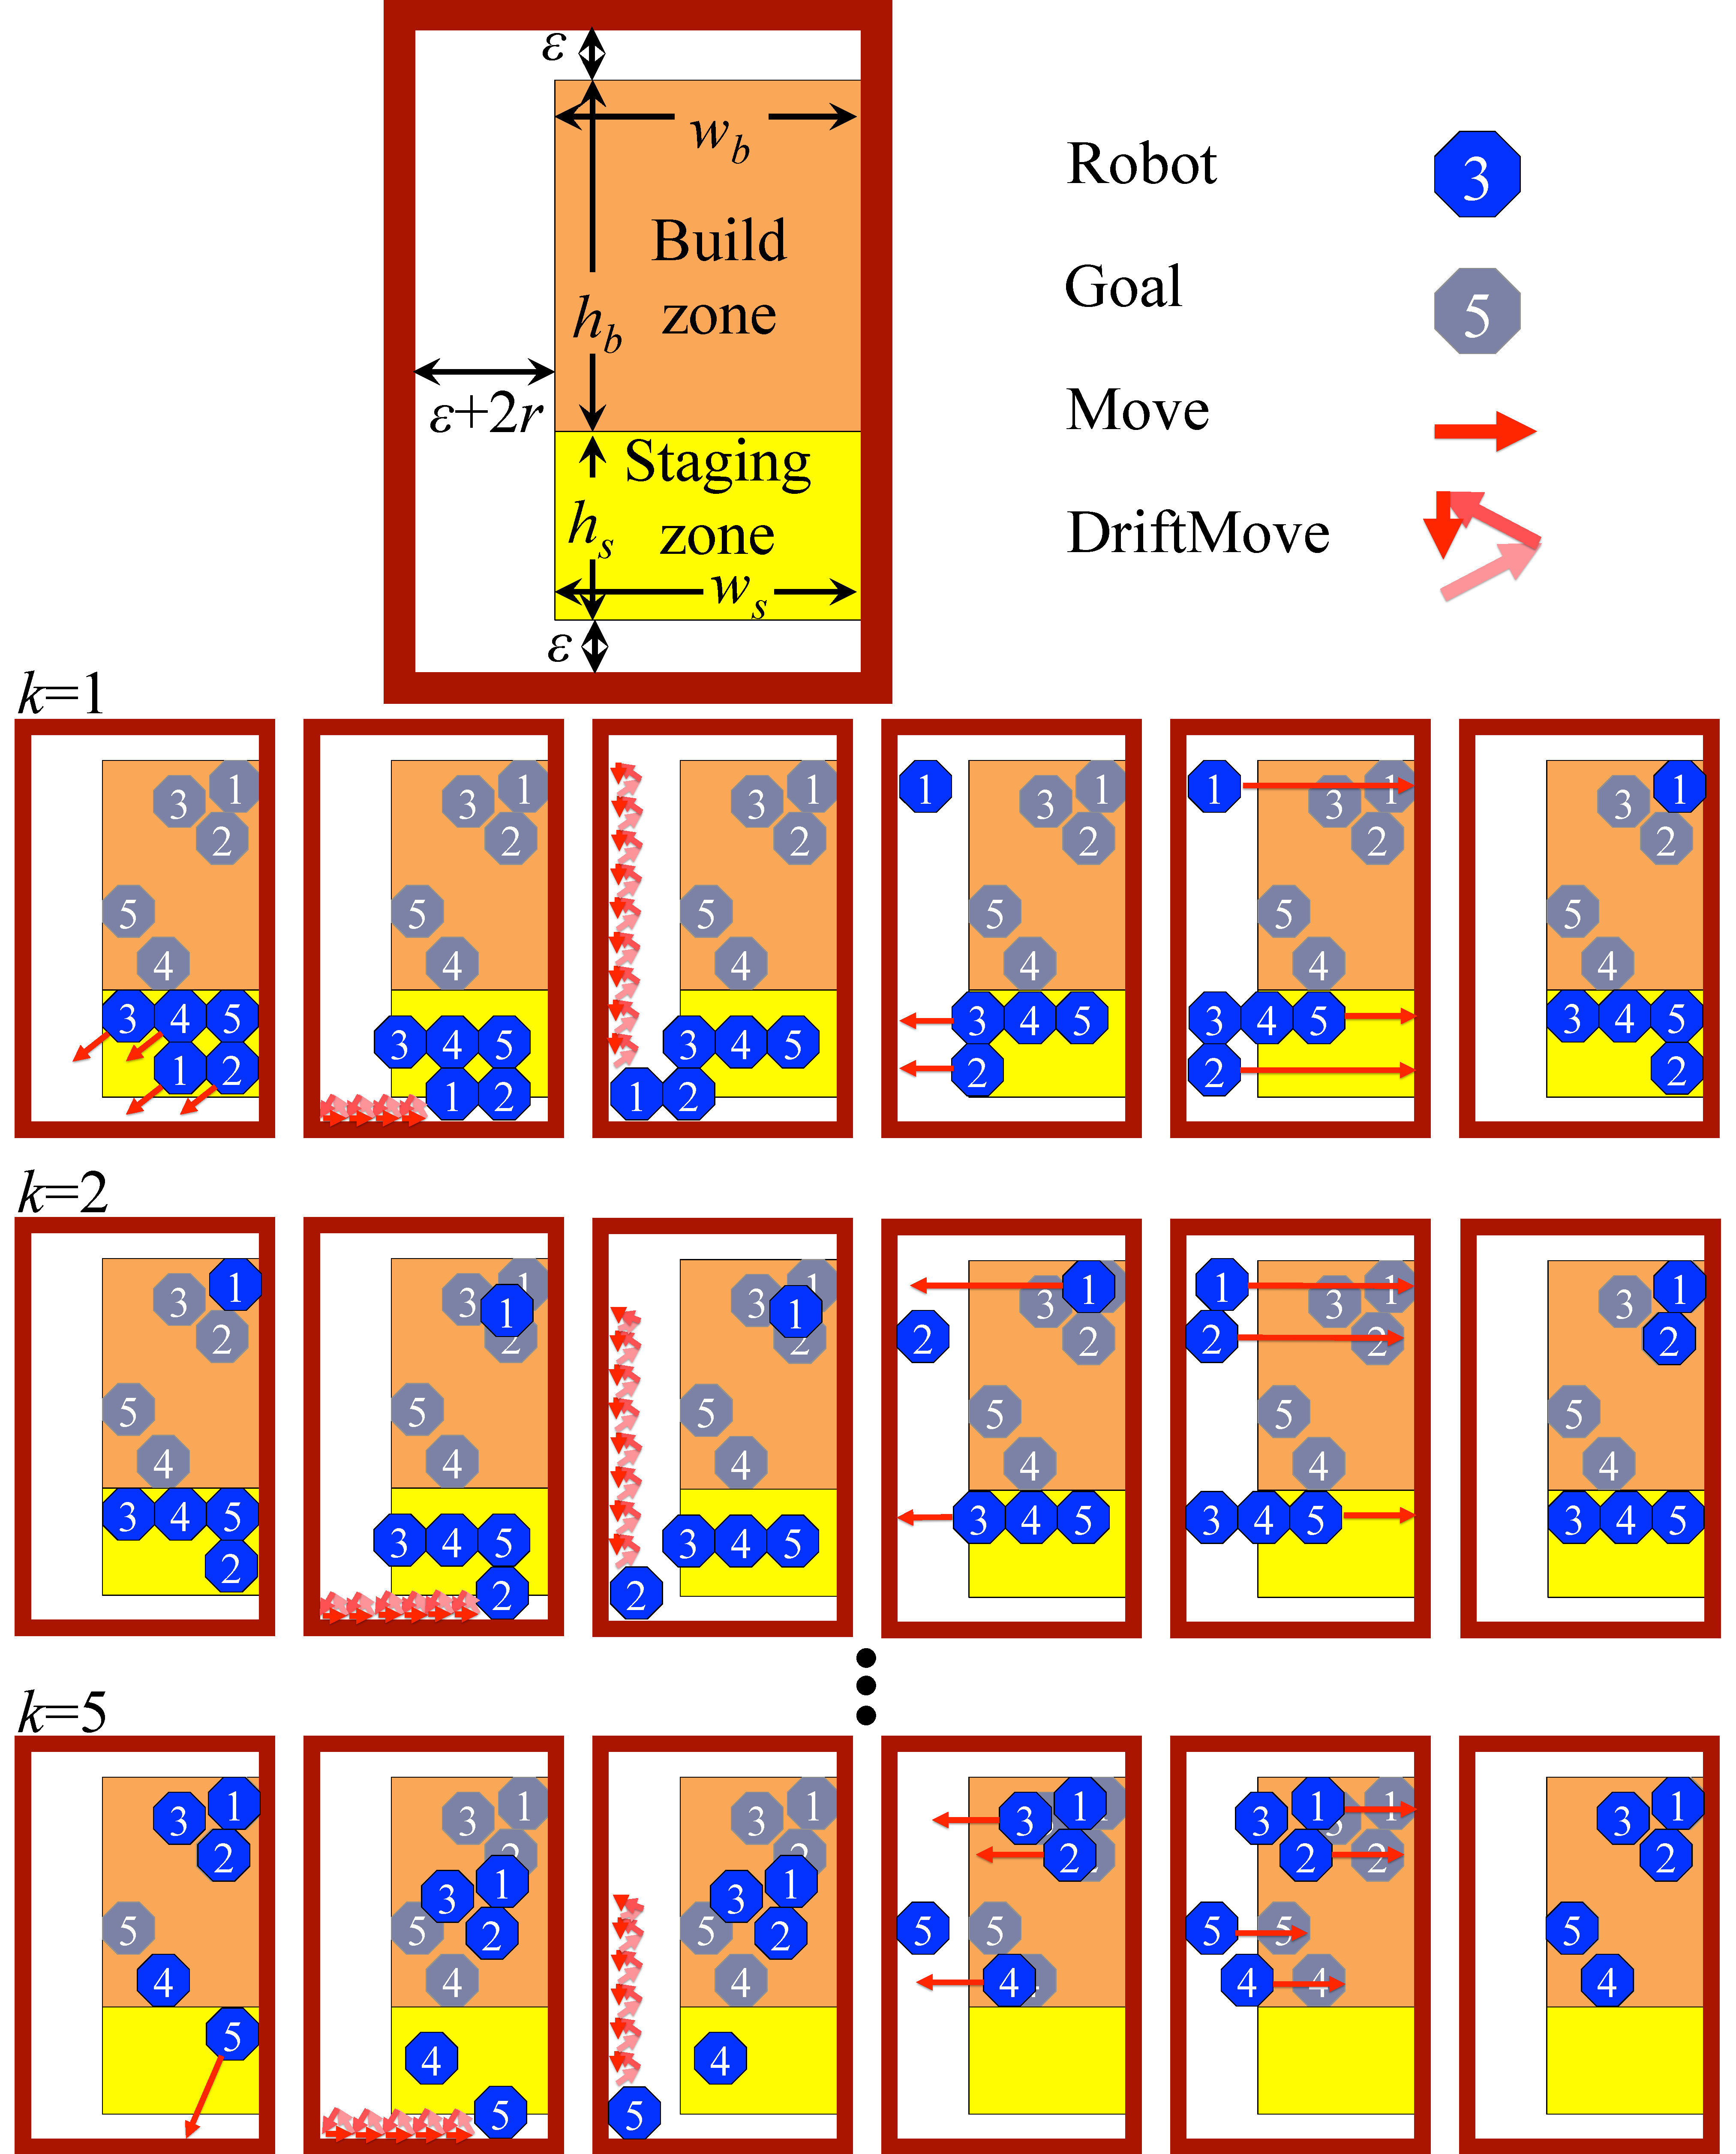
\includegraphics[width=1.0\columnwidth]{PositionNrobots.pdf}
\end{center}
\vspace{-1em}
\caption{\label{fig:construction2d}
Illustration of Alg.\ \ref{alg:PosControlNRobots}, $n$ robot position control  using wall friction.
}
\end{figure}




\subsection{AutomaticCovControl.mp4}
A closed-loop controller that steers a swarm of particles to a desired covariance,  implemented with a box2D simulator. In this video the green ellipse is the desired covariance ellipse, the red ellipse is the current covariance ellipse of the swarm and the red dot is the mean position of the robots. Robots follow the algorithm to achieve the desired values for $\sigma_{goalxy}$, $\sigma_x^2$ and $\sigma_y^2$.

%%%%%%%%%%%%%%%%%%%%%%%%%%%%%
\section{ Algorithm for generating desired $y$ spacing between two robots using wall friction}\label{sec:2robotWallFriction}
\begin{algorithm}
\caption{GenerateDesired$y$-spacing($s_1,s_2,e_1,e_2,L$)}\label{alg:YControl}
\begin{algorithmic}[1]
\Require Knowledge of starting $(s_1,s_2)$ and ending $(e_1,e_2)$ positions of  two robots. 
$(0,0)$ is bottom corner, $s_1$ is rightmost robot, 
 $L$ is length of the walls. Current position of the robots are $(r_1,r_2)$.
\Ensure   $ r_{1x} - r_{2x}  \equiv s_{1x} - s_{2x} $   %$\Delta y(t) \equiv \Delta y(0)$ 
\State $ \Delta s_y  \gets s_{1y} - s_{2y} $
\State $ \Delta e_y \gets e_{1y} - e_{2y} $
\State $ r_1 \gets s_1$, $ r_2 \gets s_2$
\If {$\Delta e_y < 0 $ }
\State $ m \gets ( L-\max( r_{1y},r_{2y}) ,0)   $ \Comment{Move to top wall}
\Else 
\State  $ m \gets ( -\min( r_{1y},r_{2y}),0 )    $ \Comment{Move to bottom wall}
\EndIf
\State $m  \gets  m + (0, -\min( r_{1x},r_{2x} ))$ \Comment{Move to left}
\State $ r_1 \gets r_1+m$, $ r_2 \gets r_2+m$ \Comment{Apply move}
\If {$\Delta e_y - (r_{1y} - r_{2y} ) > 0 $}
\State $ m \gets (\min(|\Delta e_y - \Delta s_y |, L- r_{1y}), 0)$  \Comment{Move top}
\Else
\State $ m \gets (-\min(|\Delta e_y - \Delta s_y |, r_{1y}), 0)$\Comment{Move bottom}
\EndIf 
\State $m  \gets  m + (0, \epsilon)$ \Comment{Move right}
\State $ r_1 \gets r_1+m$, $ r_2 \gets r_2+m$ \Comment{Apply move}
\State $\Delta r_y = r_{1y} - r_{2y}$
\If {$\Delta r_y \equiv \Delta e_y$} 
\State   $ m \gets (e_{1x}-r_{1x}, e_{1y}-r_{1y})$
\State $ r_1 \gets r_1+m$, $ r_2 \gets r_2+m$ \Comment{Apply move}
\State  \Return $(r_1,r_2)$
\Else   
\State \Return GenerateDesired$y$-spacing($r_1,r_2,e_1,e_2,L$)
\EndIf
\end{algorithmic}
\end{algorithm}



%%%%%%%%%%%%%%%%%%%%%%%%%%%
\section{Calculations for modeling swarm as fluid in a simple planar workspace}\label{sec:fluidInPlanarRegion}
Two workspaces are used, a square and a circular workspace.

\subsection{Square Workspace}
This section provides formulas for the mean, variance,  covariance and correlation of a very large swarm of robots as they move inside a square workplace under the influence of gravity pointing in the direction $\beta$. The swarm is large, but the robots are small in comparison, and together cover an area of constant volume $A$. Under a global input such as gravity, they flow like water, moving to a side of the workplace and forming a polygonal shape. The workspace is 

The range of possible angles for the global input angle $\beta $ is [0,2$\pi $). In this range of angles, the swarm assumes eight different polygonal shapes. The shapes alternate between triangles and trapezoids when the area $A$$<$1/2, and alternate between squares with one corner removed and trapezoids when $A$$>$1/2.

Two representative formulas are attached, the outline of the swarm shapes in \eqref{tab:SquareRobotRegions} and $\bar{x}(\beta,A)$ in \eqref{tab:SquareXMean}.




\begin{figure}[h]
\begin{center}
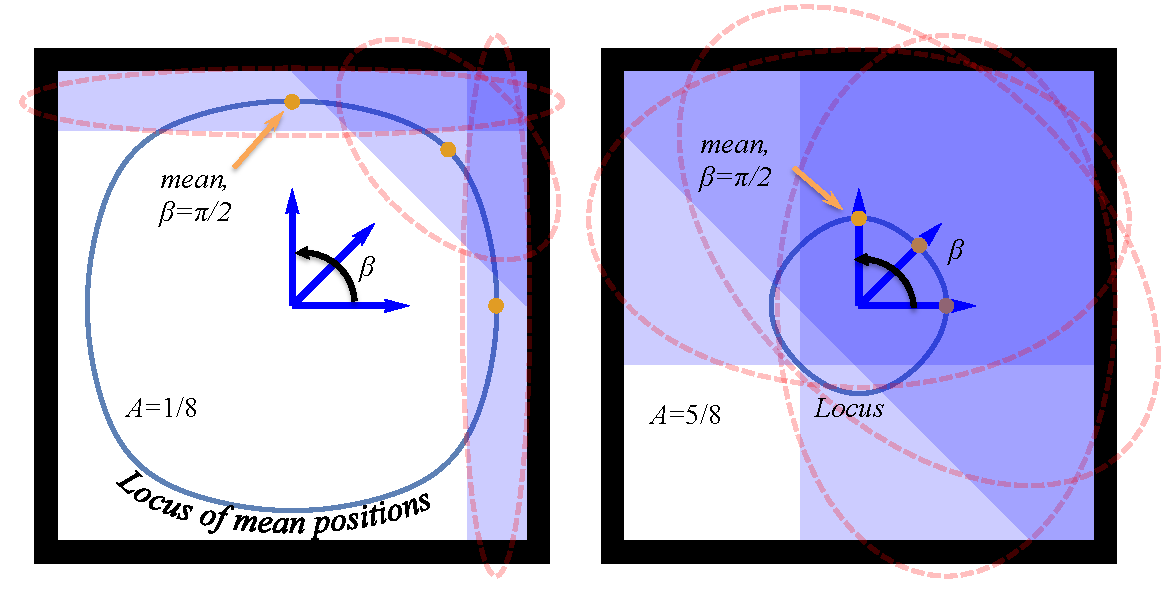
\includegraphics[width=\columnwidth]{SquarePlotPositions.pdf} 
\caption{A swarm in a square workspace under a constant global input assumes either a triangular or a trapezoidal shape if $A<1/2$.  If $A>1/2$ the swarm is either a squares with one corner removed or a trapezoidal  shape.}
\label{fig:friction}
\end{center}
\end{figure} 

\begin{table*}
\begin{align}
\bar{x}(\beta,A) = A\leq \frac{1}{2}: &\begin{cases}
 -\frac{\tan ^2(\beta )}{24 A}-\frac{A}{2}+1 & 0\leq \beta \leq \tan ^{-1}(2 A)\lor 2 \pi -\tan ^{-1}(2 A)<\beta \leq 2 \pi  \\
 1-\frac{1}{3} \sqrt{2} \sqrt{A \tan (\beta )} & \tan ^{-1}(2 A)<\beta \leq \frac{\pi }{2}-\tan ^{-1}(2 A) \\
 \frac{\cot (\beta )}{12 A}+\frac{1}{2} & \frac{\pi }{2}-\tan ^{-1}(2 A)<\beta \leq \tan ^{-1}(2 A)+\frac{\pi }{2} \\
 \frac{1}{3} \sqrt{2} \sqrt{-A \tan (\beta )} & \tan ^{-1}(2 A)+\frac{\pi }{2}<\beta \leq \pi -\tan ^{-1}(2 A) \\
 \frac{\tan ^2(\beta )}{24 A}+\frac{A}{2} & \pi -\tan ^{-1}(2 A)<\beta \leq \tan ^{-1}(2 A)+\pi  \\
 \frac{1}{3} \sqrt{2} \sqrt{A \tan (\beta )} & \tan ^{-1}(2 A)+\pi <\beta \leq \frac{3 \pi }{2}-\tan ^{-1}(2 A) \\
 \frac{1}{2}-\frac{\cot (\beta )}{12 A} & \frac{3 \pi }{2}-\tan ^{-1}(2 A)<\beta \leq \tan ^{-1}(2 A)+\frac{3 \pi }{2} \\
 1-\frac{1}{3} \sqrt{2} \sqrt{-A \tan (\beta )} & \tan ^{-1}(2 A)+\frac{3 \pi }{2}<\beta \leq 2 \pi -\tan ^{-1}(2 A) \\
\end{cases} \nonumber\\
\frac{1}{2}<A<1:&\begin{cases}
 -\frac{\tan ^2(\beta )}{24 A}-\frac{A}{2}+1 & 0\leq \beta \leq \tan ^{-1}\left(\frac{1}{2},1-A\right)\lor 2 \pi -\tan ^{-1}\left(\frac{1}{2},1-A\right)<\beta \leq 2 \pi  \\
 \frac{2 \sqrt{2} \sqrt{(1-A) \tan (\beta )} (A-1)+3}{6 A} & \tan ^{-1}\left(\frac{1}{2},1-A\right)<\beta \leq \frac{\pi }{2}-\tan ^{-1}\left(\frac{1}{2},1-A\right) \\
 \frac{6 A+\cot (\beta )}{12 A} & \frac{\pi }{2}-\tan ^{-1}\left(\frac{1}{2},1-A\right)<\beta \leq \tan ^{-1}\left(\frac{1}{2},1-A\right)+\frac{\pi }{2} \\
 \frac{-2 \sqrt{2} \sqrt{(A-1) \tan (\beta )} (A-1)+6 A-3}{6 A} & \tan ^{-1}\left(\frac{1}{2},1-A\right)+\frac{\pi }{2}<\beta \leq \pi -\tan ^{-1}\left(\frac{1}{2},1-A\right) \\
 \frac{\tan ^2(\beta )}{24 A}+\frac{A}{2} & \pi -\tan ^{-1}\left(\frac{1}{2},1-A\right)<\beta \leq \tan ^{-1}\left(\frac{1}{2},1-A\right)+\pi  \\
 \frac{2 \sqrt{2} \sqrt{(1-A) \tan (\beta )} (1-A)+6 A-3}{6 A} & \tan ^{-1}\left(\frac{1}{2},1-A\right)+\pi <\beta \leq \frac{3 \pi }{2}-\tan ^{-1}\left(\frac{1}{2},1-A\right) \\
 \frac{1}{2}-\frac{\cot (\beta )}{12 A} & \frac{3 \pi }{2}-\tan ^{-1}\left(\frac{1}{2},1-A\right)<\beta \leq \tan ^{-1}\left(\frac{1}{2},1-A\right)+\frac{3 \pi }{2} \\
 \frac{2 \sqrt{2} \sqrt{(A-1) \tan (\beta )} (A-1)+3}{6 A} & \tan ^{-1}\left(\frac{1}{2},1-A\right)+\frac{3 \pi }{2}<\beta \leq 2 \pi -\tan ^{-1}\left(\frac{1}{2},1-A\right) \\
\end{cases}
 \nonumber \\
A=1: &\frac{1}{2}
\end{align}
\protect\caption{$\bar{x}$ in a unit-square workspace}
\label{tab:SquareXMean}
\end{table*}



\begin{table*}
\tiny
\begin{align}
\text{RobotRegion}(\beta,A)= \nonumber 
A\leq \frac{1}{2}:&
\begin{cases}
 \left(
\begin{array}{cc}
 1 & 0 \\
 1 & 1 \\
 -A-\frac{\tan (\beta )}{2}+1 & 1 \\
 -A+\frac{\tan (\beta )}{2}+1 & 0 \\
\end{array}
\right) & 0\leq \beta \leq \tan ^{-1}(2 A)\lor 2 \pi -\tan ^{-1}(2 A)<\beta \leq 2 \pi  \\
 \left(
\begin{array}{cc}
 1 & 1 \\
 1-\sqrt{2} \sqrt{A \tan (\beta )} & 1 \\
 1 & 1-\sqrt{2} \sqrt{A \cot (\beta )} \\
\end{array}
\right) & \tan ^{-1}(2 A)<\beta \leq \frac{\pi }{2}-\tan ^{-1}(2 A) \\
 \left(
\begin{array}{cc}
 1 & 1 \\
 0 & 1 \\
 0 & -A+\frac{\cot (\beta )}{2}+1 \\
 1 & -A-\frac{\cot (\beta )}{2}+1 \\
\end{array}
\right) & \frac{\pi }{2}-\tan ^{-1}(2 A)<\beta \leq \tan ^{-1}(2 A)+\frac{\pi }{2} \\
 \left(
\begin{array}{cc}
 0 & 1 \\
 \sqrt{2} \sqrt{-A \tan (\beta )} & 1 \\
 0 & 1-\sqrt{2} \sqrt{-A \cot (\beta )} \\
\end{array}
\right) & \tan ^{-1}(2 A)+\frac{\pi }{2}<\beta \leq \pi -\tan ^{-1}(2 A) \\
 \left(
\begin{array}{cc}
 0 & 0 \\
 0 & 1 \\
 A-\frac{\tan (\beta )}{2} & 1 \\
 A+\frac{\tan (\beta )}{2} & 0 \\
\end{array}
\right) & \pi -\tan ^{-1}(2 A)<\beta \leq \tan ^{-1}(2 A)+\pi  \\
 \left(
\begin{array}{cc}
 0 & 0 \\
 0 & \sqrt{2} \sqrt{A \cot (\beta )} \\
 \sqrt{2} \sqrt{A \tan (\beta )} & 0 \\
\end{array}
\right) & \tan ^{-1}(2 A)+\pi <\beta \leq \frac{3 \pi }{2}-\tan ^{-1}(2 A) \\
 \left(
\begin{array}{cc}
 0 & 0 \\
 1 & 0 \\
 1 & A-\frac{\cot (\beta )}{2} \\
 0 & A+\frac{\cot (\beta )}{2} \\
\end{array}
\right) & \frac{3 \pi }{2}-\tan ^{-1}(2 A)<\beta \leq \tan ^{-1}(2 A)+\frac{3 \pi }{2} \\
 \left(
\begin{array}{cc}
 1 & 0 \\
 1-\sqrt{2} \sqrt{-A \tan (\beta )} & 0 \\
 1 & \sqrt{2} \sqrt{-A \cot (\beta )} \\
\end{array}
\right) & \tan ^{-1}(2 A)+\frac{3 \pi }{2}<\beta \leq 2 \pi -\tan ^{-1}(2 A) \\
\end{cases}
 %%%%%%%%%%%%%%%%%%%%%%%%%%%%%%%%%%
\nonumber \\
\frac{1}{2}<A<1:&
\begin{cases}
 \left(
\begin{array}{cc}
 1 & 0 \\
 1 & 1 \\
 (1-A)-\frac{\tan (\beta )}{2} & 1 \\
 (1-A)+\frac{\tan (\beta )}{2} & 0 \\
\end{array}
\right) & 0\leq \beta \leq \tan ^{-1}\left(\frac{1}{2},1-A\right)\lor 2 \pi -\tan ^{-1}\left(\frac{1}{2},1-A\right)<\beta \leq 2 \pi  \\
 \left(
\begin{array}{cc}
 1 & 0 \\
 1 & 1 \\
 0 & 1 \\
 0 & \sqrt{2} \sqrt{(1-A) \cot (\beta )} \\
 \sqrt{2} \sqrt{(1-A) \tan (\beta )} & 0 \\
\end{array}
\right) & \tan ^{-1}\left(\frac{1}{2},1-A\right)<\beta \leq \frac{\pi }{2}-\tan ^{-1}\left(\frac{1}{2},1-A\right) \\
 \left(
\begin{array}{cc}
 0 & 1 \\
 1 & 1 \\
 1 & (1-A)-\frac{\cot (\beta )}{2} \\
 0 & (1-A)+\frac{\cot (\beta )}{2} \\
\end{array}
\right) & \frac{\pi }{2}-\tan ^{-1}\left(\frac{1}{2},1-A\right)<\beta \leq \tan ^{-1}\left(\frac{1}{2},1-A\right)+\frac{\pi }{2} \\
 \left(
\begin{array}{cc}
 1 & 1 \\
 0 & 1 \\
 0 & 0 \\
 1-\sqrt{2} \sqrt{-(1-A) \tan (\beta )} & 0 \\
 1 & \sqrt{2} \sqrt{-(1-A) \cot (\beta )} \\
\end{array}
\right) & \tan ^{-1}\left(\frac{1}{2},1-A\right)+\frac{\pi }{2}<\beta \leq \pi -\tan ^{-1}\left(\frac{1}{2},1-A\right) \\
 \left(
\begin{array}{cc}
 0 & 0 \\
 0 & 1 \\
 -(1-A)-\frac{\tan (\beta )}{2}+1 & 1 \\
 -(1-A)+\frac{\tan (\beta )}{2}+1 & 0 \\
\end{array}
\right) & \pi -\tan ^{-1}\left(\frac{1}{2},1-A\right)<\beta \leq \tan ^{-1}\left(\frac{1}{2},1-A\right)+\pi  \\
 \left(
\begin{array}{cc}
 1 & 0 \\
 0 & 0 \\
 0 & 1 \\
 1-\sqrt{2} \sqrt{(1-A) \tan (\beta )} & 1 \\
 1 & 1-\sqrt{2} \sqrt{(1-A) \cot (\beta )} \\
\end{array}
\right) & \tan ^{-1}\left(\frac{1}{2},1-A\right)+\pi <\beta \leq \frac{3 \pi }{2}-\tan ^{-1}\left(\frac{1}{2},1-A\right) \\
 \left(
\begin{array}{cc}
 1 & 0 \\
 0 & 0 \\
 0 & -(1-A)+\frac{\cot (\beta )}{2}+1 \\
 1 & -(1-A)-\frac{\cot (\beta )}{2}+1 \\
\end{array}
\right) & \frac{3 \pi }{2}-\tan ^{-1}\left(\frac{1}{2},1-A\right)<\beta \leq \tan ^{-1}\left(\frac{1}{2},1-A\right)+\frac{3 \pi }{2} \\
 \left(
\begin{array}{cc}
 0 & 0 \\
 1 & 0 \\
 1 & 1 \\
 \sqrt{2} \sqrt{-(1-A) \tan (\beta )} & 1 \\
 0 & 1-\sqrt{2} \sqrt{-(1-A) \cot (\beta )} \\
\end{array}
\right) & \tan ^{-1}\left(\frac{1}{2},1-A\right)+\frac{3 \pi }{2}<\beta \leq 2 \pi -\tan ^{-1}\left(\frac{1}{2},1-A\right) \\
\end{cases},\nonumber\\
%%%%%%%%%%%%%%%%%%%%%%%%%%%%%%%
A=1:&\left(
\begin{array}{cc}
 1 & 0 \\
 0 & 0 \\
 0 & 1 \\
 1 & 1 \\
\end{array}
\right)
\end{align}
\protect\caption{RobotRegions in a unit-square workspace}
\label{tab:SquareRobotRegions}
\end{table*}


\subsection{Circle Workspace}
The area under a chord of a circle is the area of a sector less the area of the triangle originating at the circle center: 
$A=S(sector)-S(triangle)=1/2 LR-1/2 C(1-h)$, thus
\begin{align}
A=(1/2)\left[LR-c(R-h)\right]
\end{align}
where $L$ is arc length, $c$ is chord length, $R$ is radius and $h$ is height. Solving for $L$ and $C$ gives
\begin{align}
L&=2 \cos ^{-1}(1-h)\\
C&=2\sqrt{h(2-h)}
\end{align}
Therefore the area under a chord is
\begin{align}
\cos ^{-1}(1-h)-(1-h) \sqrt{(2-h) h}
\end{align}

For a circular workspace, with $\beta = 0$, the variance of $x$ and $y$ are:
{\tiny
\begin{align}
&\sigma_x^2(h)=\frac{64 (h-2)^3 h^3}{144 \left(\sqrt{-(h-2) h} (h-1)+\arccos(1-h)\right)^2} +\nonumber\\
&\frac{9 \left(\sqrt{-(h-2) h} (h-1)+\arccos(1-h)\right) \left(\sin \left(4 \arcsin(1-h)\right)+4 \arccos(1-h)\right)}{144 \left(\sqrt{-(h-2) h} (h-1)+\arccos(1-h)\right)^2}
\end{align}}

{\tiny
\begin{align}
\sigma_y^2(h)=
\frac{12 \arccos(1-h)-8 \sin \left(2 \arccos(1-h)\right)+\sin \left(4 \arccos(1-h)\right)}{48 \left(\sqrt{-(h-2) h} (h-1)+\arccos(1-h)\right)}
\end{align}}

For $\beta = 0$, $\sigma_{xy}=0$. These values can be rotated to calculate $\sigma_x^2(\beta,h),\sigma_y^2(\beta,h),$ and $\sigma_{xy}(\beta,h)$.

%%%%%%%%%%%%%%%%%%%%%%%%%%%%%%
\section*{Acknowledgments}
This work was supported by the National Science Foundation under Grant No.\ \href{http://nsf.gov/awardsearch/showAward?AWD_ID=1553063}{ [IIS-1553063]}.

%%%%%%%%%%%%%%%
%% Use plainnat to work nicely with natbib. 
\bibliographystyle{plainnat}
\footnotesize
\bibliography{IEEEabrv,ShapingSwarmFrictionSharedInput}
\end{document}





\end{document}